\documentclass[12pt,a4paper]{article}
\usepackage[utf8]{inputenc}
\usepackage[portuguese]{babel}
\usepackage[margin=2cm]{geometry}
%\setlength{\parindent}{13pt}
\usepackage{listings,mathptmx,amsfonts,amsmath,amssymb,amsthm}
\linespread{1.3}% equals 1.5 of line spacing

\usepackage[font=footnotesize,labelfont=bf,tableposition=top]{caption}

%\usepackage[backend=bibtex,citestyle=numeric-comp,bibstyle=ieee,sorting=none,minbibnames=5,maxbibnames=5,defernumbers=true,firstinits=true]{biblatex}

\usepackage{subcaption,mathtools,float,cite,lipsum,bm,physics,pythontex,caption}
%\usepackage[colorlinks]{hyperref}
\usepackage{sectsty,isotope,xcolor}
\usepackage{graphicx}

%\hypersetup{linkcolor=blue}
%\hypersetup{citecolor=blue}

\usepackage[colorlinks = true,
	linkcolor = blue,
	urlcolor  = blue,
	citecolor = blue,
	anchorcolor = blue]{hyperref}

\usepackage[nameinlink,capitalize]{cleveref}
\usepackage[bottom]{footmisc}

\title{\textbf{Estudo Computacional do Nelfinavir\\incorporado na HIV-1 Protease}}
\author{\textbf{António Cesário}\\\\%
	Faculdade de Ciências da Universidade do Porto\\%
	Mestrado em Física Experimental\\%
	Bioquímica Computacional%\\%
	}
\date{23 de janeiro de 2022}

\begin{document}
	\maketitle
	\begin{abstract}
		Neste trabalho foram exploradas os primeiros passos com rumo à simulação de sistemas biológicos, tendo sido abordada teoria, trabalho computacional e vários métodos de análise da dados.
	
		A incorporação do Nelfinavir na HIV-1 protease foi o nosso objeto de estudo e foi realizada uma pequena simulação de 120 ps de Dinâmica Molecular, que se mostrou termodinamicamente estável, embora não se tenha conseguido chegar a uma estrutura convergida.
		
		A análise de dados foi bastante diversificada, permitindo-me aprender maneiras diferentes de extrair vários tipos de informação das estruturas obtidas, desde comprimentos e ângulos de ligação das pontes de hidrogénio do sistema às funções de distribuição radial de moléculas de água de certos átomos em resíduos de referência.
	\end{abstract}
	\newpage
	
\section{Introdução}
	%Visão geral sobre o que vou falar nesta secção.
\subsection{Inibidores da HIV-1 protease}
	%Alguns destes pontos são para ser discutidos no abstract.
	%Falar da proteína em si e quais as suas funções, pq é que danificá-la para a propagação/infeção da sida, o que é um inibidor, extra: como é que foi implementado experimentalmente este inibidor no artigo usado extra: origem da ideia de usar este inibidor
	A Protease do HIV-1 é uma enzima responsável por um passo essencial no ciclo de vida do vírus HIV. Para que as proteínas do HIV-1 desempenharem as suas funções, é necessário que elas sejam clivadas em pontos específicos. Dada a especificidade deste processo, foram procuradas formas de interferir com ele, afim de interromper o ciclo de vida do vírus.
	
	Neste relatório foi abordado um dos métodos desenvolvidos para concretizar esta ideia, incorporando o inibidor \textit{Nelfinavir} na estrutura da protease.
	
	Em primeiro irei apresentar algum fundamento teórico para explicar a física subjacente aos cálculos computacionais. Depois mostro como representar a estrutura estudada e explico como foram executadas as simulações computacionais. Por último irei apresentar os resultados das simulações e explorar vários métodos de análise dos dados obtidos.
	
\section{Fundamento Teórico}
	A base para a entendermos como se comportam estes sistemas biológicos está em estabelecer modelos computacionais que nos permitam simular propriedades de interesse. Nesta secção apresento alguns destes métodos e refiro ideias que encontrei durante a minha pesquisa e tenha achado interessantes.
	
	Os princípios físicos utilizados dependem de modelo para modelo, sendo os mais importantes derivados de Mecânica Molecular, Dinâmica Molecular e Mecânica Quântica Molecular. Como o sistema estudado possui centenas de átomos, as simulações baseadas em Mecânica Quântica não são passíveis de se concluírem em tempo útil, pelo que neste trabalho apenas foram estudados apenas os primeiros dois métodos computacionais.
	
\subsection{Mecânica Molecular}\label{sec:MM}
	O método mais comum para descrever a energia de um sistema biológico serve-se de potenciais empíricos derivados da Mecânica Molecular.	Se considerarmos um sistema de $N$ átomos, a sua energia potencial, $U\left(r_{1}, r_{2}, \ldots, r_{N}\right)$, pode ser descomposta como a soma de de interações a uma partícula, duas partículas, e assim sucessivamente:
	\begin{equation}
		U\left(r_{1}, r_{2}, \ldots, r_{N}\right) = \sum_{i=1}^{N} U\left(r_{i}\right)+\sum_{i=1}^{N} \sum_{j>i}^{N} U\left(r_{i}, r_{j}\right)+\sum_{i=1}^{N} \sum_{j>i}^{N} \sum_{k>j>i}^{N} U\left(r_{i}, r_{j}, r_{k}\right)+\ldots
		\label{eq:intro:Udecomp}
	\end{equation}
	onde $r_i$ representa o vetor posição do átomo $i$. Aproximações são então impostas para simplificar o problema. O termo de primeira ordem, $U\left(r_{i}\right)$, está associado às interações com campos externos ao sistema, pelo que normalmente não é considerado.
	
	Os termos de segunda e terceira ordem, por outro lado, contêm as interações mais energéticas do sistema, pelo que estes são os mais estudados, enquanto que os de quarta ordem e superior são desprezados. No entanto, como as interações a três partículas são muito dispendiosas a nível computacional, foram encontradas maneiras de omitir estes termos reajustando os campos de forças e os parâmetros que governam as interações a duas partículas.
	
	O problema inicial foi então reduzido a entender como é que o sistema se comporta face ao potencial:
	\begin{equation}
		U\left(r_{1}, r_{2}, \ldots, r_{N}\right) \approx \sum_{i=1}^{N} \sum_{j>i}^{N} U\left(r_{i}, r_{j}\right)
		\label{eq:intro:Usecond-order}
	\end{equation}
	onde cada termo pode ser decomposto em vários potenciais empíricos, caracterizando interações diferentes, resumidas abaixo e esquematizadas na \cref{fig:intro:inters}.

	\begin{figure}[h]
		\centering
		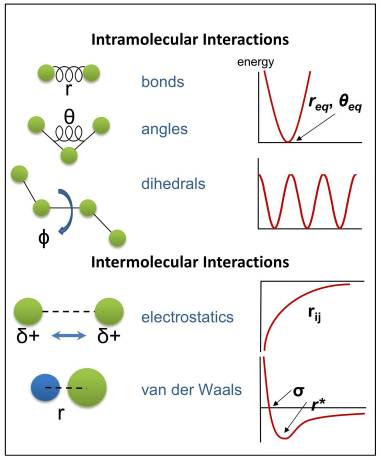
\includegraphics[width=0.5\textwidth]{images/interactions.jpeg}
		\caption{Resumo da origem das interações mais importantes para o termo potencial da \cref{eq:intro:Usecond-order}. À direita encontram-se as formas genéricas dos respetivos potenciais. Imagem de \cite{cheathamMolecularModelingNucleic2001}.}
		\label{fig:intro:inters}
	\end{figure}

\subsubsection{Interações Intramoleculares}
	As interações intramoleculares descrevem a estrutura covalente de uma molécula, de onde se distinguem a energia de ligação, os ângulos de ligação, e os diedros/torção.
	
	A energia de ligação entre dois átomos é um termo harmónico, resultante da expansão do potencial num polinómio de Taylor, até segunda ordem, em função da distância entre as duas partículas, $r$. No entanto, esta aproximação não prevê corretamente a energia das ligações  para desvios significativos da posição de equilíbrio, como esquematizado na \cref{fig:intro:harmonic-deviation}. Para contornar este problema podem ser incluídos termos de maior ordem do polinómio de Taylor.
	
	Analogamente, a energia do ângulo de ligação também apresenta um comportamento harmónico, com origem nas (pequenas) oscilações do ângulo que dois átomos fazem com um terceiro, $\theta$.

	\begin{figure}[h]
		\centering
		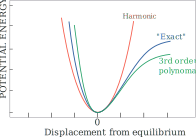
\includegraphics[width=0.5\textwidth]{images/harmonic-deviation.png}
		\caption{Validade das aproximações de primeira e segunda ordem em $r$ e em $\theta$ na determinação da energia de ligação entre duas partículas. Imagem de \cite{2021Harmonic}.}
		\label{fig:intro:harmonic-deviation}
	\end{figure}
	 
	 A energia de torção tem origem na rotação das ligações e varia sinusoidalmente com o ângulo de torção, $\phi$. As interações intramoleculares podem, portanto, ser escritas na forma:
	\begin{equation}
		U_{\text {intra }}\left(r_i,r_j\right)=U_{\text {intra }}\left(r,\theta,\phi\right)= K_{\textrm{lig}}\left(r-r_{e q}\right)^{2}+ K_{\theta}\left(\theta-\theta_{e q}\right)^{2}+ \sum_{n} \frac{V_{n}}{2}[1+\cos (n \phi-\gamma)]
	\end{equation}
	onde $r_{eq}$, $\theta_{eq}$, e $\gamma$ são parâmetros de equilíbrio da geometria, e os parâmetros $K_\textrm{lig}$, $K_\theta$ e $V_n$ são constantes de força, que caracterizam a dependência da energia face os desvios à geometria de equilíbrio. 
	
	O somatório em $n$ no termo de torção diz-nos que podemos ter vários ângulos de rotação estáveis, onde o $n$ está associado à periodicidade/simetria do sistema, que determina o de mínimos de energia contidos entre $0$ e $2\pi$.
	
	As interações intramoleculares entre duas partículas do sistema são, portanto, caracterizadas pelo conjunto de parâmetros referidos, tipicamente sob a assunção de que o campo de forças é transferível de vizinhança para vizinhança, ou seja: uma ligação C-C num propano deve de ser semelhante a C-C em butano. Porém, esta transferibilidade nem sempre é possível, pelo que existem campos de forças que só podem ser aplicados num conjunto restrito de sistemas. Também existem casos em que as ligações são especificadas tendo em conta um terceiro átomo, por exemplo: um conjunto de parâmetros se em C-C um dos C's estiver ligado a um H e outro conjunto se esse C estiver ligado a um S.
	
	Os comprimentos e ângulos de ligação são determinados experimentalmente por cristalografia (como difração de neutrões, ou outras técnicas de espectroscopia), com constantes de força inferidas a partir de outras experiências de micro-ondas ou infravermelhos, por exemplo. Os termos de torção, por outro lado, são muito mais difíceis de determinar experimentalmente, por envolverem a interação de quatro partículas, embora a ligação que estejamos a analisar seja só entre duas. Estes parâmetros costumam ser os últimos a ser determinados, obtidos pela conjugação de dados experimentais, por exemplo através de Ressonância Magnética Nuclear, e cálculos de Mecânica Quântica \cite{weinerNewForceField1984,cheathamMolecularModelingNucleic2001,cornellSecondGenerationForce1995}.

\subsubsection{Interações Intermoleculares}
	As interações intermoleculares envolvem forças de maior alcance. Quando dois átomos $i$ e $j$ com cargas parciais $q_i$ e $q_j$, respetivamente, se encontram a uma distância $r_{ij}$, a sua energia potencial eletroestática é dada pela Lei de Coulomb:
	\begin{equation}
		U_C\left(r_i,r_j\right) = \dfrac{q_iq_j}{4\pi\epsilon}\dfrac{1}{r_{ij}}
	\end{equation}
	onde $\epsilon$ é a permitividade elétrica do meio. Para ter uma descrição mais completa da energia do sistema, é introduzido o potencial de Lennard-Jones:
	\begin{equation}
		U_{\text {LJ}}=\frac{A_{i j}}{r_{i j}^{12}}-\frac{B_{i j}}{r_{i j}^{6}}
	\end{equation}
	onde o primeiro termo representa a repulsão das nuvens eletrónicas de $i$ e $j$, e o segundo é um termo de atração resultante de forças de dispersão de eletrões. Para simular este tipo de interações também é necessário determinar os parâmetros $q_i,q_j,A_{ij},B_{ij}$ \cite{cornellSecondGenerationForce1995}.\paragraph{}
	
	O problema de Mecânica Molecular da \cref{eq:intro:Udecomp} foi, portanto, reduzido à minimização do potencial:
	
	\begin{equation}
		\begin{gathered}
			U=\sum_{\textrm{bonds}} K_{\textrm{lig}}^{ij}\left(r_{ij}-r_{e q}^{ij}\right)^{2}+\sum_{\text {angles }} K_{\theta}^{ij}\left(\theta_{ij}-\theta_{e q}^{ij}\right)^{2}+\\
			\sum_{\text {dihedrals}} \sum_{n} \frac{V_{n}^{ij}}{2}[1+\cos (n \phi_{ij}-\gamma^{ij})]+\sum_{\text {non-bond }}\left[\frac{A_{i j}}{R_{i j}^{12}}-\frac{B_{i j}}{R_{i j}^{6}}+\frac{q_{i} q_{j}}{\varepsilon R_{i j}}\right]
		\end{gathered}
	\end{equation}
	que corresponde à forma como estão parametrizados os campos de força AMBER, que possuem informação sobre milhares de combinações possíveis de parâmetros, que são introduzidos nesta equação para determinar, por exemplo, a configuração de distâncias, ângulos e torções intramoleculares que minimizam a energia de uma molécula. Mais informações sobre estes campos de força podem ser encontradas na \href{https://ambermd.org/AmberModels.php}{página web} e no seu \href{https://ambermd.org/doc12/Amber21.pdf#page=264}{manual de 2021}.
	
	Existem, no entanto, várias desvantagens nestes métodos. Para além de termos que determinar e
	ricamente uma grande parte dos campos de forças, a Mecânica Molecular não nos permite obter com confiança a conformação de menor energia de um sistema. Isto acontece devido à elevada complexidade da superfície de potencial e o grande número de graus de liberdade. Assim, não é possível determinar o mínimo global do potencial sem uma amostragem exaustiva do imenso espaço das configurações possíveis. % - ver \cref{fig:intro:miniprob}.
	É neste contexto que surgem outros métodos de simulação alternativos/complementares como a Dinâmica Molecular \cite{cheathamMolecularModelingNucleic2001,galindo-murilloMolecularModelingNucleic2014} ou até mesmo simulações de Monte-Carlo \cite{tenekedjievApplicationsMonteCarlo2011}.
%	\begin{figure}[h]
%		\centering
%		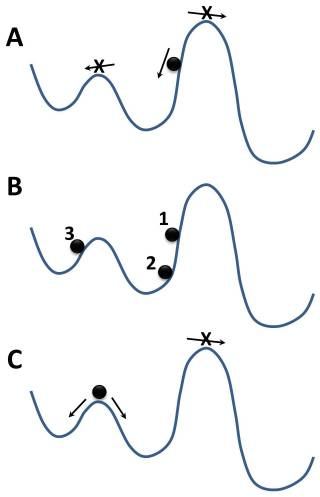
\includegraphics[width=0.2\textwidth]{images/minimization.jpeg}
%		\caption{Image from \cite{cheathamMolecularModelingNucleic2001}.}
%		\label{fig:intro:miniprob}
%	\end{figure}
	
\subsection{Dinâmica Molecular}
	As simulações de dinâmica molecular baseiam-se na integração das equações clássicas de movimento, as equações de Newton, para todos os átomos no sistema. A simulação inicia-se com a atribuição estocástica de velocidades às $N$ partículas, baseada na distribuição de Boltzmann para uma dada temperatura T tal que:
	\begin{equation}
		\frac{1}{2} \sum_{i}^{N} m_{i} v_{i}^{2}=\frac{3 N k_{\mathrm{B}} T}{2}
	\end{equation}
	
	Seja $U_{ij}$ o potencial entre os átomos $i$ e $j$ como vimos na Sec. (\ref{sec:MM}), a força que $j$ exerce sobre $i$ é dada por
	\begin{equation}
		F_i=-\nabla_{i} \sum_{j}^{N} U_{i j}
	\end{equation}
	logo, pela segunda lei de Newton:
	\begin{equation}
		m_{i} \frac{d^{2} r_{i}}{d t^{2}}=-\nabla_{i} \sum_{j}^{N} U_{i j}
		\label{eq:DM:segundaNewton}
	\end{equation}

	A dinâmica é então propagada pela integração numérica da \cref{eq:DM:segundaNewton}, de onde se extrairá a velocidade (integrar 1x) e a posição (integrar 2x) de cada uma das partículas do sistema. Os métodos numéricos tipicamente implementados são o das velocidades de Verlet e o \textit{leapfrog} \cite{newman2013computational}. Este último algoritmo foi o utilizado nas nossas simulações, onde a cada iteração são calculadas as forças, posições e velocidades de cada átomo, pelo que é necessário escolher um bom compromisso entre tempo de computação e precisão, atendendo sempre ao facto de que a escala temporal do nosso passo de integração tem que ser menor que o fenómeno mais rápido que queremos estudar.
	Os cálculos das forças podem ser muito exigentes, pelo que certos algoritmos podem optar por simplificar $U_{ij}$ relativamente à Mecânica Molecular. Também é conveniente distinguir que os campos de força mencionados anteriormente na Sec. (\ref{sec:MM}) estão otimizados para a estrutura e não para dinâmica.
	
	A estabilidade das simulações está intimamente ligada ao passo de integração, que por sua vez está associado à frequência esperada da dinâmica. As ligações que envolvem hidrogénio são muito rápidas, sugerindo-nos passos de integração extremamente pequenos, $<$ 1 fs, para ter uma boa amostragem da dinâmica. Felizmente, o algoritmo SHAKE \cite{ryckaertNumericalIntegrationCartesian1977} permite-nos restringir graus de liberdade dessas ligações tal que seja possível utilizar tempos de integração maiores.
	
	Uma limitação significativa da DM é o tempo de simulação necessário para o sistema ultrapassar grandes barreiras de potencial. À temperatura ambiente, barreiras de 1 e 5 kcal/mol conseguem ser ultrapassadas em ps e ns de simulação, respetivamente, enquanto que para 10 kcal/mol já são necessárias simulações da ordem dos $\mu$s \cite{cheathamMolecularModelingNucleic2001}. Isto impede as simulações de concluírem uma amostragem completa do espaço de estados em tempo útil de computação.
	
\subsection{RMSD - análise da convergência da estrutura}
	Depois de todos estes métodos de simulação, precisamos de ter uma forma quantitativa de avaliar a convergência dos resultados. Como as posições dos átomos variam de uma iteração para a outra, podemos obter os desvios sofridos por cada átomo em \textit{snapshots} diferentes do sistema e representar a média destes desvios. A isto dá-se o nome de ``Root Mean Square Deviation'' (RMSD) e tem a forma:
	\begin{equation}
		R M S D(v, w)=\sqrt{\frac{1}{N} \sum_{i=1}^{N}\left(\left(v_{i x}-w_{i x}\right)^{2}+\left(v_{i y}-w_{i y}\right)^{2}+\left(v_{i z}-w_{i z}\right)^{2}\right)}
	\end{equation}
	onde $v_i$ e $w_i$ são as posições do átomo $i$ nos \textit{snapshots} $v$ e $w$, respetivamente.
	
	\paragraph{}Estando estabelecidos os princípios teóricos necessários para compreender as bases por detrás dos cálculos computacionais, estamos agora em condições de explorar o trabalho computacional e de simulação.
\section{Preparar e Visualizar a Estrutura}
	A estrutura inicial foi obtida no website de RCSB Protein Data Bank, onde se encontra identificada pelo nome \textit{1ohr}, que pode visitar diretamente através \href{https://www.rcsb.org/structure/1OHR}{deste link}.
	
	O primeiro passo foi procurar desvendar a informação contida em \verb|1ohr.pdb|. Ao abrir o ficheiro com um editor de texto, podemos encontrar a descrição do sistema em estudo estruturada como na \cref{fig:vis:pdb-print}, onde está expressa a informação relativa a cada átomo que constitui o sistema. Identificamos pelo menos duas cadeias, A e B, divididas no ficheiro pela linha inciada por \verb|TER|. Conseguimos também observar a composição e distribuição dos elementos do resíduo PRO da cadeia B, identificado como o seu primeiro resíduo. Com base nestas coordenadas e associações a resíduos, cadeias, entre outros, será possível estabelecer representações gráficas do sistema com o auxílio do \textit{free software} VMD (Visual Molecular Dynamics) \cite{HUMP96}.
	
	\begin{figure}[h]
		\centering
		\includegraphics[width=0.8\textwidth]{images/pdb-print.png}
		\caption{Secção da informação contida em 1ohr.pdb. As colunas correspondem a: (1) Identificação do tipo de campo; (2,3) número e nome do átomo no sistema; (4,6) nome e número do resíduo; (5) cadeia; (7-9) coordenadas $(x,y,z)$; (10) fator de ocupação; (11) fator temperatura; (12) elemento químico. Podemos observar a transição da cadeia A para a B e os dados referentes ao primeiro resíduo (PRO) da cadeia B.}%\verb|1ohr.pdb|.}
		\label{fig:vis:pdb-print}
	\end{figure}
	
	Na \cref{fig:vis:original-pdb} temos representada a estrutura inicial, onde estão destacadas as cadeias (A e B), as flaps das cadeias, o inibidor e os asparatos catalíticos.

	\begin{figure}[h]
		\centering
		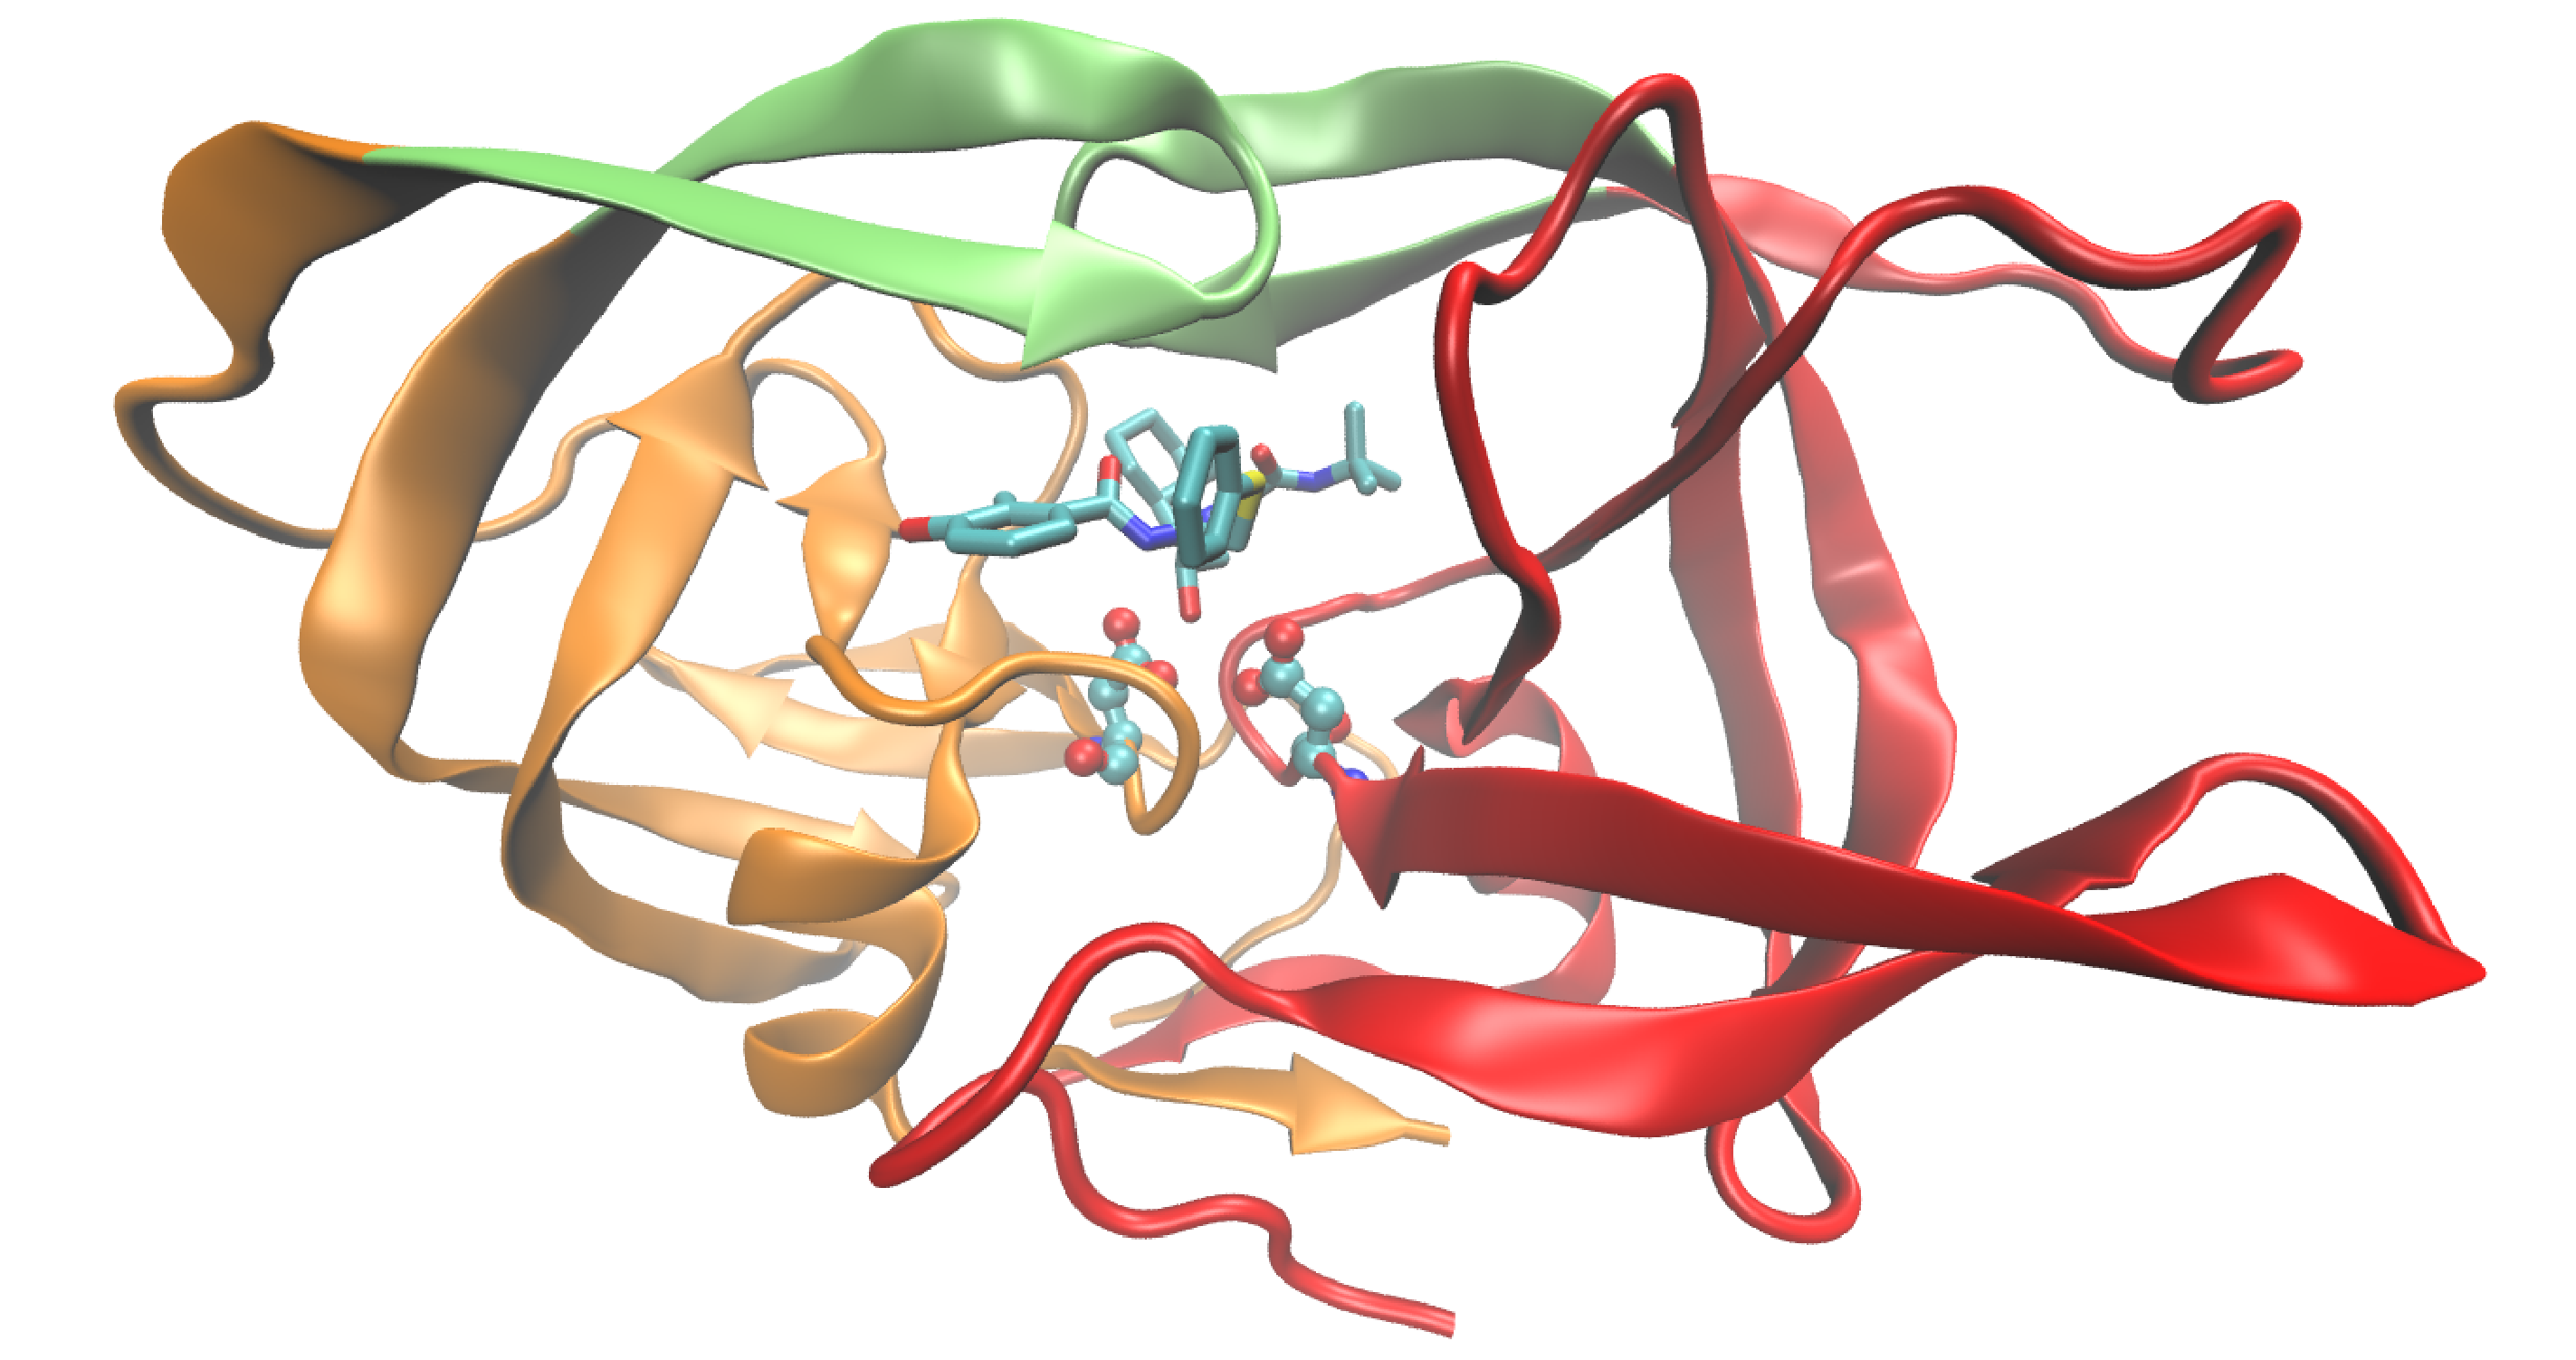
\includegraphics[width=0.8\textwidth]{images/1ohr-chains.pdf}
		\caption{Ilustração da estrutura inicial. A proteína está representada no modo \textit{NewCartoon} e dividida nas cadeias A (laranja + verde) e B (vermelho + verde), cujas \textit{flaps} foram destacadas a verde. Abaixo das \textit{flaps} observamos o inibidor \textit{Nelfinavir}. Os resíduos ASP25 das das duas cadeias também estão visíveis abaixo do inibidor e ligadas às respetivas cadeias.}
		\label{fig:vis:original-pdb}
	\end{figure}

\subsection{Preparação do Ficheiro PDB}

	Embora tenhamos uma representação do sistema que queremos estudar, esta serve apenas como uma aproximação incical à sua estrutura. Isto deve-se ao facto destes dados terem sido obtidos experimentalmente, possivelmente em condições diferentes daquelas em que estamos interessados. É muito importante levar isto em conta porque podemos querer simular meios e/ou condições de pressão-temperatura específicos, alterando comprimentos ou ângulos de ligação e, possivelmente, quantidades termodinâmicas em que estamos interessados.
	
\subsubsection{Remover Hidrogénios}
	Como a estrutura da \cref{fig:vis:original-pdb} foi obtida por cristalografia de raios-x, uma técnica que tem origem no \textit{scattering} de raios-x na nuvem eletrónica, e o hidrogénio possui apenas um eletrão de valência, é provável que as posições detetadas para estes átomos sejam pouco precisas ou que até não tenham sido detetados todos os hidrogénios da estrutura \cite{woinskaHydrogenAtomsCan2016}. O próximo passo foi, portanto, remover todas as linhas em \verb|1ohr.pdb| onde se encontram átomos de H, resultando no ficheiro \verb|1ohr-no-H.pdb|. Estes átomos serão posteriormente adicionados pelo AMBER.

\subsubsection{Identificar Interações no Inibidor}\label{sec:vis:inibidor}
	Para lidar com elementos estruturais diferentes, distinguir por exemplo uma prolina (PRO) de uma glutamina (GLN), o AMBER recorre a bibliotecas que possuem modelos destas estruturas básicas. No entanto, o inibidor Nelfinavir, que designaremos por 1UN, não está presente nestas bibliotecas, pelo que teremos que o adicionar ao AMBER antes de prosseguir com as simulações. A criação dos \textit{scripts} adequados é um processo complexo, pelo que os professores simplesmente nos forneceram os ficheiros necessários já preparados: \verb|1UN.mod| e \verb|1UN.prepc|.
	
\subsubsection{ASP25 Protonado}
	Como é referido em \cite{soaresDatasetShowingImpact2016,perezSubstrateRecognitionHIV12010}, o sistema constituído pela protease e o inibidor só é estável se um dos dois ácidos aspárticos (ASP25) for protonado. Para o AMBER interpretar um deles como tal, alterou-se \verb|ASP| (desprotonado) para \verb|ASH| (protonado) na cadeia A.
	
%	\begin{equation}
%		\mathrm{pH} - \mathrm{pKa} = \log\dfrac{\left[A\right]}
%		{\left[AH^+\right]}
%	\end{equation}
%	logo, se pKa $>$ pH, teremos $\left[AH^+\right] > \left[A\right]$, pelo que o ácido estará protonado. 
	
	
	%\# Explicar o porquê de ter que protonar o ASP. Não esotu a conseguir entender qual deles protonar porque não entendo qual é a diferença de o fazer 
	%\textit{Q: Porquê?? Qual é o nosso objetivo? Pq é que fazemos as simulações de dinâmica molecular? Queremos determinar as propriedades termodinâmicas da molécula para ver a estabilidade e outras trips que o inibidor tem sobre a protase? Ok, mas o quê ao certo? E porque é que não confiamos nos dados do pdb inicial? Porque é que assumimos que o que foi obtido experimentalmente está errado enquanto que e confiamos em vez nos nossos cálculos de dinâmica molecular, baseados e campos de forças e etc aproximados?} 
	
	
\section{Simulações Computacionais}
	%Adicionar o inibidor à biblioteca local de compostos do amber, talvez mostrar onde é guardada essa biblioteca, adicionar as águas (solvatação), neutralizar as cargas, falar daquela trip do pH e pKa nas caudas, minimização de energia para convergir as posições dos hidrogénios e não sei mais quê, dinâmica molecular para subir a temperatura e depois para relaxar o volume
	
	A concretização destas simulações passa pela elaboração de \textit{scripts} escritos especificamente para as várias funções de AMBER utilizadas. Para facilitar a partilha do código utilizado e o apresentar de uma maneira conveniente, disponibilizei todo o trabalho computacional num \href{https://github.com/cesarium/biochem-report}{repositório de GitHub}, permitindo também a reprodução dos resultados obtidos.
	
	%Irei começar por resumir esta parte computacional indicando todos os passos que seguimos. Depois disso irei explicar como cada um deles foi realizado.\textbf{\#basear-me no soares 2016}	
	Antes de submeter o sistema às simulações de dinâmica, ainda é necessário neutralizá-lo, adicionar um solvente, e proceder à minimização da sua energia por mecânica molecular. Estes cálculos foram realizados através dos pacotes \verb|xleap| e \verb|sander| do AMBER-12, cujo manual pode ser encontrado \href{https://ambermd.org/doc12/Amber12.pdf}{neste link}. Foram usados os campos de forças AMBER FF03 \cite{duanPointchargeForceField2003,zhangWellbalancedForceField2019}, para simular certos parâmetros dos resíduos, e o \href{https://ambermd.org/antechamber/gaff.html}{GAFF } (\textit{General Amber Force Field}), que nos permite estudar um grande número de moléculas orgânicas compostas por C, N, O, H, S, P, F, Cl, Br e I. Os ficheiros referidos na Sec.(\ref{sec:vis:inibidor}) também tiveram que ser dados como \textit{input}.
	
	Num à parte, e porque queria ter uma noção do tipo de informação necessária para construir um campo de forças eficiente, encontrei um repositório no GitHub com os ficheiros \href{https://github.com/choderalab/ambermini/blob/master/share/amber/dat/leap/cmd/oldff/leaprc.ff03}{leaprc.ff03} e \href{https://github.com/choderalab/ambermini/blob/master/share/amber/dat/leap/cmd/leaprc.gaff}{leaprc.gaff}, semelhantes aos que foram carregados pelo \verb|xleap|. Estes dependem, por sua vez, de outros mais extensos como \href{https://github.com/choderalab/ambermini/blob/master/share/amber/dat/leap/parm/gaff.dat}{gaff.dat} e \href{https://github.com/choderalab/ambermini/blob/master/share/amber/dat/leap/lib/all_aminoct03.lib}{all\_aminoct03.lib}, respetivamente, que possuem uma longa lista de dados que caracterizam as interações/ligações entre vários átomos/estruturas. Todos estes ficheiros têm que ser lidos pelo AMBER, e encontram-se algures nos sub-diretórios da variável local \verb|$AMBERHOME|. Muita informação útil também pode ser encontrada na \href{https://ambermd.org/AmberModels.php}{página web} e no \href{https://ambermd.org/doc12/Amber21.pdf#page=264}{manual de 2021} do AMBER, que já foram referidos na Sec. (\ref{sec:MM}).
	
\subsection{Adição de um Solvente}
	O sistema atual encontra-se em vácuo, pelo que precisamos de simular uma situação mais próxima daquelas em que a molécula se encontra na realidade, adicionando, por exemplo, uma vizinhança constituída por água.
	
	Antes de adicionar a água é necessário neutralizar o sistema. Com o \verb|xleap| adicionaram-se iões de Cl$^-$ e/ou Na$^+$, conforme determinado pelo programa, e logo depois, introduziu-se no sistema uma caixa de águas (explícitas) com dimensões tais que as distâncias do exterior da proteína às paredes da caixa sejam no mínimo 12\AA. Os valores tipicamente usados para as dimensões da caixa encontra-se entre $8-12$\AA, quando condições fronteira periódicas são aplicadas aos cálculos \cite{galindo-murilloMolecularModelingNucleic2014}, que serão incluídas a seguir na mecânica e dinâmica moleculares. O valor escolhido é um \textit{trade-off} entre precisão e custo computacional, que aumentam com as dimensões da caixa. Deste processo resultam os ficheiros seguintes: \verb|prot-nelf.pdb|, \verb|prot-nelf.prmtop|, e \verb|prot-nelf.inpcrd|. O primeiro é simplesmente o \verb|.pdb| anterior mas com a caixa de águas e os iões neutralizadores. No \href{https://ambermd.org/FileFormats.php#topology}{prmtop} encontram-se os parâmetros do campo de forças e a topologia do sistema. Esta informação permanecerá inalterada ao longo das simulações. Por último, \verb|inpcrd| possui as coordenadas dos vários átomos e até das velocidades, quando pedido para dar \textit{print} nos cálculos de dinâmica molecular. Ao longo das simulações estas posições irão evoluir, cada uma resultando num novo conjunto de coordenadas.	
		
\subsection{Mecânica Molecular - Minimização da Energia}
	% Queria encontrar uma maneira de introduzir o abundância de mínimos locais abaixo dessa energia resultaria em estruturas muito afastadas da realidade ou instáveis.
	A introdução de certa forma grosseira das águas e dos iões pelo \verb|xleap| coloca o sistema num estado de elevada energia e com as ligações entre os átomos muito pouco otimizadas, pelo que precisamos de fazer as águas e os iões reagir à presença da molécula molécula. Se iniciássemos neste ponto a dinâmica molecular, os ângulos e distâncias interatómicas resultariam em forças irrealisticamente elevadas em vários átomos. Para as simulações de dinâmica, esta condição inicial faria com que esses elementos se deslocassem significativamente da sua posição na estrutura inicial, tendo energia suficiente para se aproximar significativamente de outros átomos, transmitindo-os energia para estes também se deslocaram consideravelmente da sua posição inicial. Este efeito em cadeia resultaria em conformações finais instáveis e incorretas \cite{cheathamMolecularModelingNucleic2001}.
	
	Aqui entra o processo de minimização de energia por mecânica molecular, utilizado para aproximar o sistema atual do seu estado fundamental. Este método não tem a capacidade de determinar com precisão a conformação convergida, mas idealmente irá aproximá-la o suficiente para a podermos alcançar por dinâmica molecular \cite{cheathamMolecularModelingNucleic2001,galindo-murilloMolecularModelingNucleic2014}.\paragraph{}
	
	O sistema passou por três processos de minimização: no primeiro relaxou-se as posições e geometria das moléculas de água; em segundo foram otimizadas as posições dos hidrogénios; em terceiro relaxou-se a posição de todos os átomos.
	
	Cada um destes processos começou com 250 iterações de \textit{steepest descent} e acabou com 250 de um algoritmo de gradiente conjugado. Foram admitidas condições fronteira periódicas e usou-se um raio de corte de 10\AA \ para interações não ligantes, ou seja, entre moléculas distintas.
	
\subsection{Dinâmica Molecular - Equilibração e Produção}
	%particular observable property (e.g., temperature, pressure, volume, potential energy).
	%Equilibration is necessary in molecular dynamics simulations to relax structural distortions and remove large forces that may bias the dynamics. This means that equilibration is necessary to thermalize the system to put a comparable amount of kinetic energy into each degree of freedom. When this is not done, large forces may result at the distortions that, in turn, lead to large collisions on the local scale and create local “hot spots”. These hot spots may move the structure in unrealistic ways. Therefore, the goal of the equilibration procedure is to relax the system as much as possible to avoid biasing it away from the starting geometry. This is generally done through a series of minimization and	molecular dynamics simulations where the temperature or kinetic energy is gradually increased.
	
	%on binding for the larger PNA) and that the conformation sampled by the minimization
	%is only a local minimum. In addition to being a useful tool for modeling, minimization is
	%necessary prior to running molecular dynamics simulations to relieve any large steric
	%overlap or remove strained bonds or angles that might otherwise lead to initially large
	%forces. During the dynamics, the large forces lead to large displacements, which in turn
	%may lead to more overlaps and more large displacements; this cascade of events can lead
	%to local hot spots or failure of the integrator during MD.
	
	As simulações de dinâmica molecular foram divididas em duas partes: equilibração e produção. Na equilibração, correspondendo ao ensemble canónico, o sistema foi aquecido a volume constante desde 0 K até à temperatura de produção de 310.15 K (37 $^\circ$C) ao longo de 20 ps com intervalo de integração de 1 fs. Para controlo de temperatura usou-se o termostato de Langevin com fator $\gamma = 1 \textrm{ ps}^{-1}$, que corresponde à frequência das colisões, responsáveis pela troca de energia cinética entre os átomos. Foi considerado um raio de corte de 10\AA \ para as interações não ligantes. Nesta fase pretendemos preparar o sistema para a simulação biologicamente relevante, tendo-se mantido o volume constante ao longo da simulação. Face à exigência computacional destes cálculos, eles foram realizados através do SANDER compilado em paralelo: \verb|sander.MPI|.
	
	Na produção, por outro lado, a temperatura e a pressão foram mantidas constantes, a 310.15 K e 1 bar, respetivamente, e o sistema foi evoluído ao longo de 100 ps com intervalo de integração de 1 fs. O controlo de temperatura e o raio de corte foram iguais ao da primeira dinâmica, enquanto que o controlo de pressão foi realizado através de ``MD with isotropic position scaling'' com um tempo de relaxação de 2 ps. Esta parte da DM também foi compilada pelo \verb|sander.MPI| usando 4 nodos, demorando cerca de 10h para finalizar o cálculo.
	
	Como não consegui com que cálculos tão longos corressem sem interrupção nas máquinas da FCUP (por alguma razão a sessão expirava em etapas diferentes da simulação), a partir daqui irei usar os resultados de DM dos professores.
	
\section{Análise de Dados}
	%explicar porquê que se usa apenas a última, explicar se os 120ps são suficientes para estabilizar o sistema, se acho que ele já convergiu, comparar a primeira snapshot com a última e ver como o sistema evoluiu, responder àquelas perguntas todas nos capítulos 7 e 8!! AHHHHHHHHHHHHHHHHHHHHHHHHH
	Depois de finalizados os 120 ps de dinâmica, queremos analisar como evolui o sistema neste período. O nosso primeiro objetivo é procurar saber se ocorreram alterações significativas na estrutura da proteína. Depois foi analisada a evolução das variáveis termodinâmicas e do RMSD para tirar conclusões quanto à convergência da simulação.
	
	Os dados utilizados nesta análise obtiveram-se pelos resultados obtidos pela simulação de 120 ps dos professores. Os professores escolheram alterar no seu \verb|.pdb| a protonação do ASP25 da cadeia B para ASH, enquanto que acima eu fiz-lo para a cadeia A.
	
\subsection{Variações Estruturais}\label{sec:variacoes-estruturais}
	Na \cref{fig:an:conformations} encontra-se representada a sua estrutura quaternária no primeiro e último \textit{frames} da fase de produção, a verde e laranja, respetivamente. Os \textit{loops} correspondem às regiões mais desorganizadas e flexíveis, pelo que são as estruturas secundárias que mais variaram no decorrer da simulação. Por outro lado, as conformações $\alpha$ e $\beta$ sofreram poucas alterações, um possível indicador de que a simulação não correu tempo suficiente para se observarem variações estruturais significativas do sistema.
	
	\begin{figure}[h]
	\centering
	\begin{subfigure}[b]{0.64\textwidth}
		\centering
		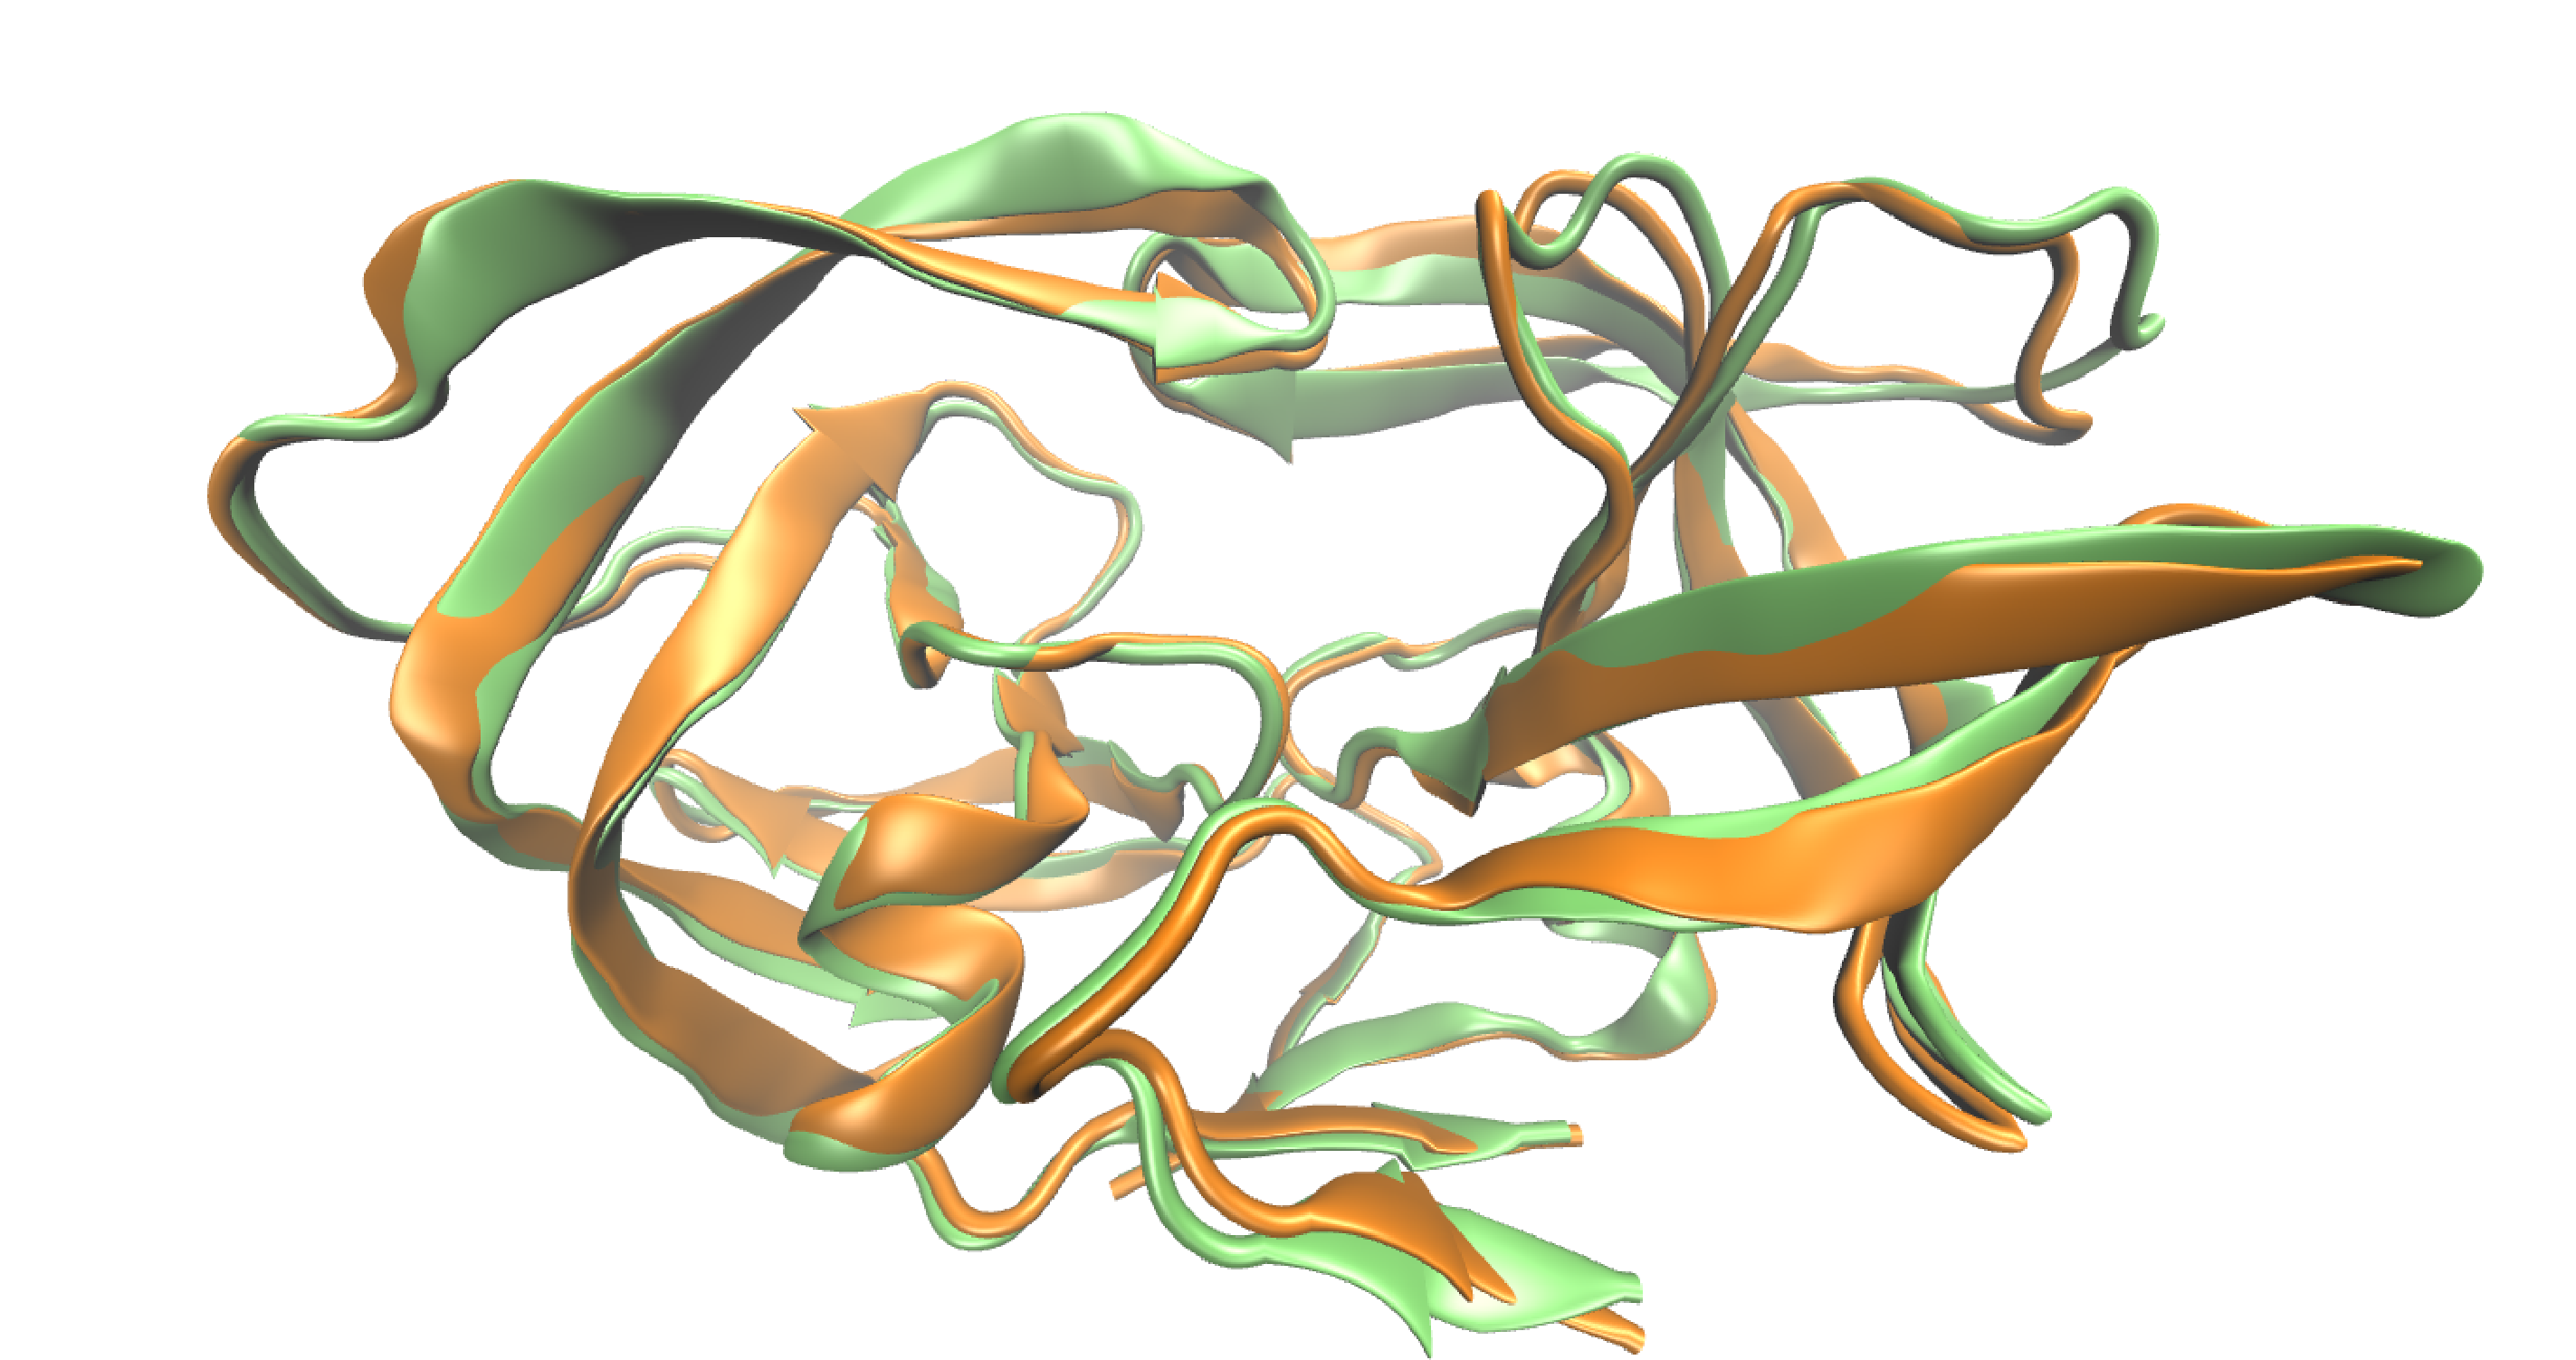
\includegraphics[width=\textwidth]{images/conformations.pdf}
		\caption{}
		\label{fig:an:conformations}
	\end{subfigure}
	\begin{subfigure}[b]{0.34\textwidth}
		\centering
		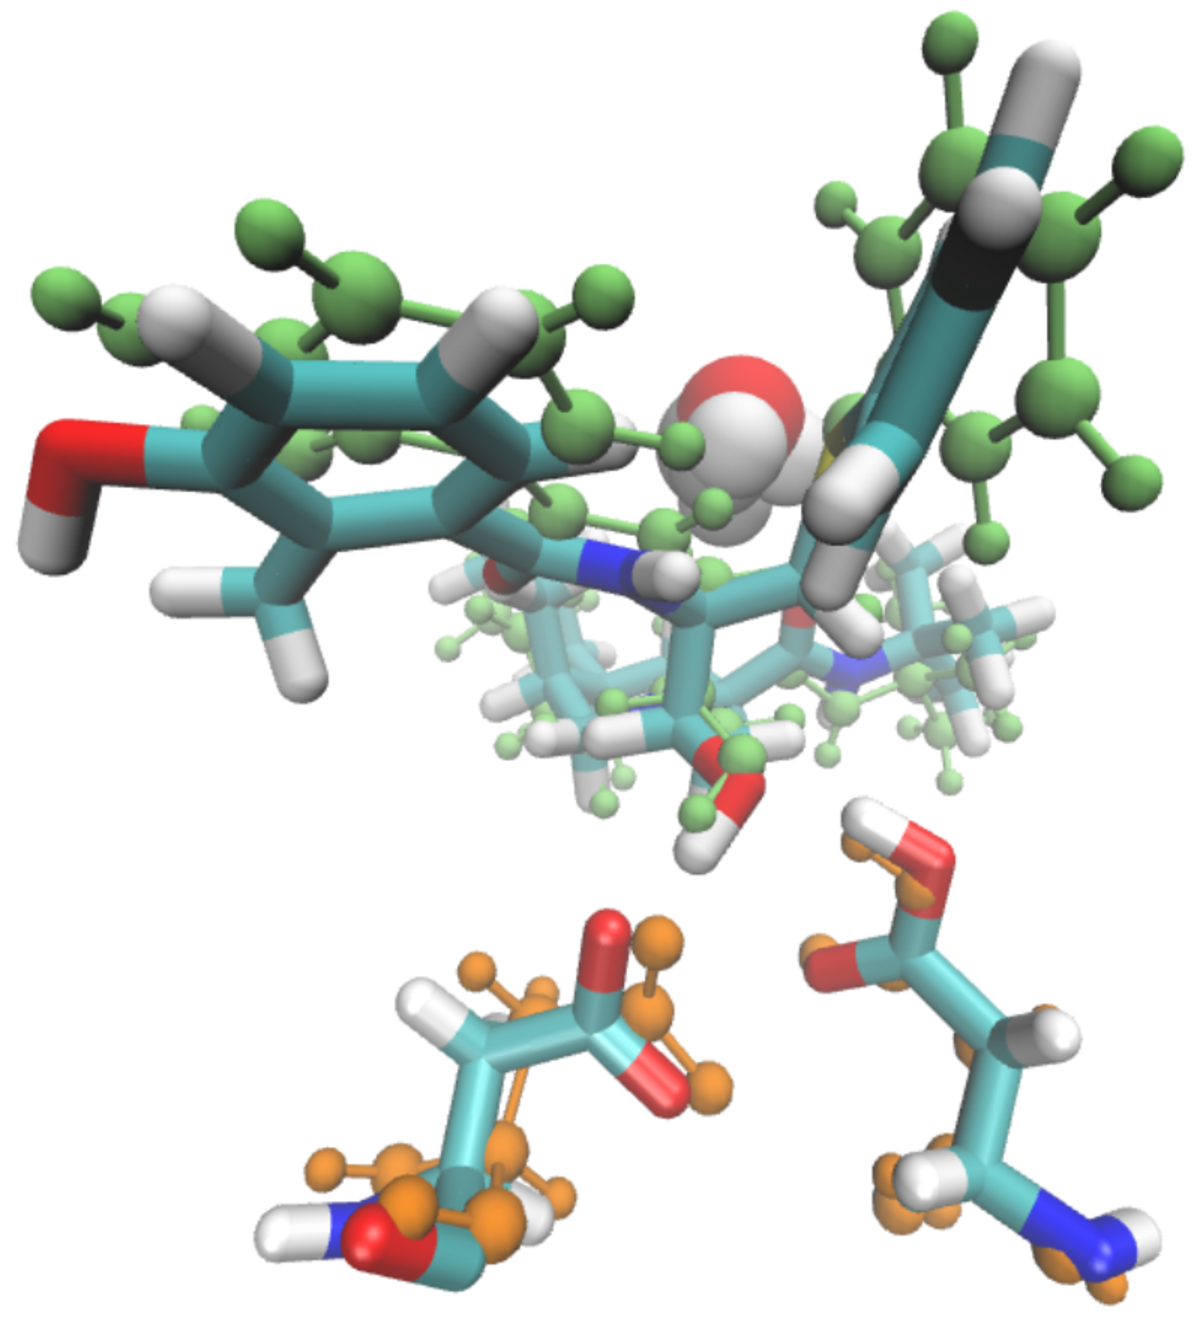
\includegraphics[width=\textwidth]{images/1UN-comparison-crop.pdf}
		\caption{}
		\label{fig:an:1UN-comparison}
	\end{subfigure}
	\caption{\textbf{(a)} Estrutura quaternária antes e depois da fase de produção, a verde e laranja, respetivamente. As estruturas foram alinhadas através da funcionalidade ``Extensions - Analysis - RMSD Trajectory Tool'' do VMD. \textbf{(b)} Comparação das posições relativas do inibidor, da água catalítica e dos resíduos ASP 25 antes e depois da fase de produção. As moléculas representadas a múltiplas cores correspondem às obtidas depois da produção. A laranja e verde estão representados os ASP25 e o nelfinavir, respetivamente, no início da produção. Aproximadamente ao centro da imagem, por cima do inibidor, consegue-se observar uma molécula de água a cores e, aproximadamente na mesma posição, uma outra molécula de água a cinzento.}
	\end{figure}

	Uma outra representação que pode ser importante é a das posições relativas dos ASP25 e do inibidor relativamente à proteína. Na \cref{fig:an:1UN-comparison} estão representados os resíduos ASP25 (\verb|resid = 25 124|), a água catalítica (\verb|resid = 25|) e o inibidor (\verb|resid = 199|) antes e depois da produção. Como vemos, todas estas estruturas encontram-se muito próximas das suas posições iniciais, tendo sofrido algumas deformações estruturais. Atendendo às Figs. (\ref{fig:vis:original-pdb},\ref{fig:an:conformations}), como as posições das \textit{flaps} e do \textit{backbone} se mantiveram aproximadamente as mesmas, então podemos concluir que as estruturas representadas na \cref{fig:an:1UN-comparison} se mantêm aproximadamente na localização inicial, pelo que o inibidor continua associado à enzima e no seu centro ativo. 
	
	A molécula de água estrutural também foi observada com um pouco mais de detalhe, tendo-se verificado que manteve uma posição praticamente fixa ao longo da simulação. Além disso, usou-se o VMD para determinar as pontes de hidrogénio em que esta água intervém, tendo-se observado duas com os resíduos ILE50 e duas com o inibidor - ver \cref{fig:an:wat205-vmd} - cujos comprimentos foram extraídos pelo VMD para todas as iterações da produção - \cref{fig:an:wat205-plot}.
	
	\begin{figure}[h]
	\begin{subfigure}[b]{0.48\textwidth}
		\centering
		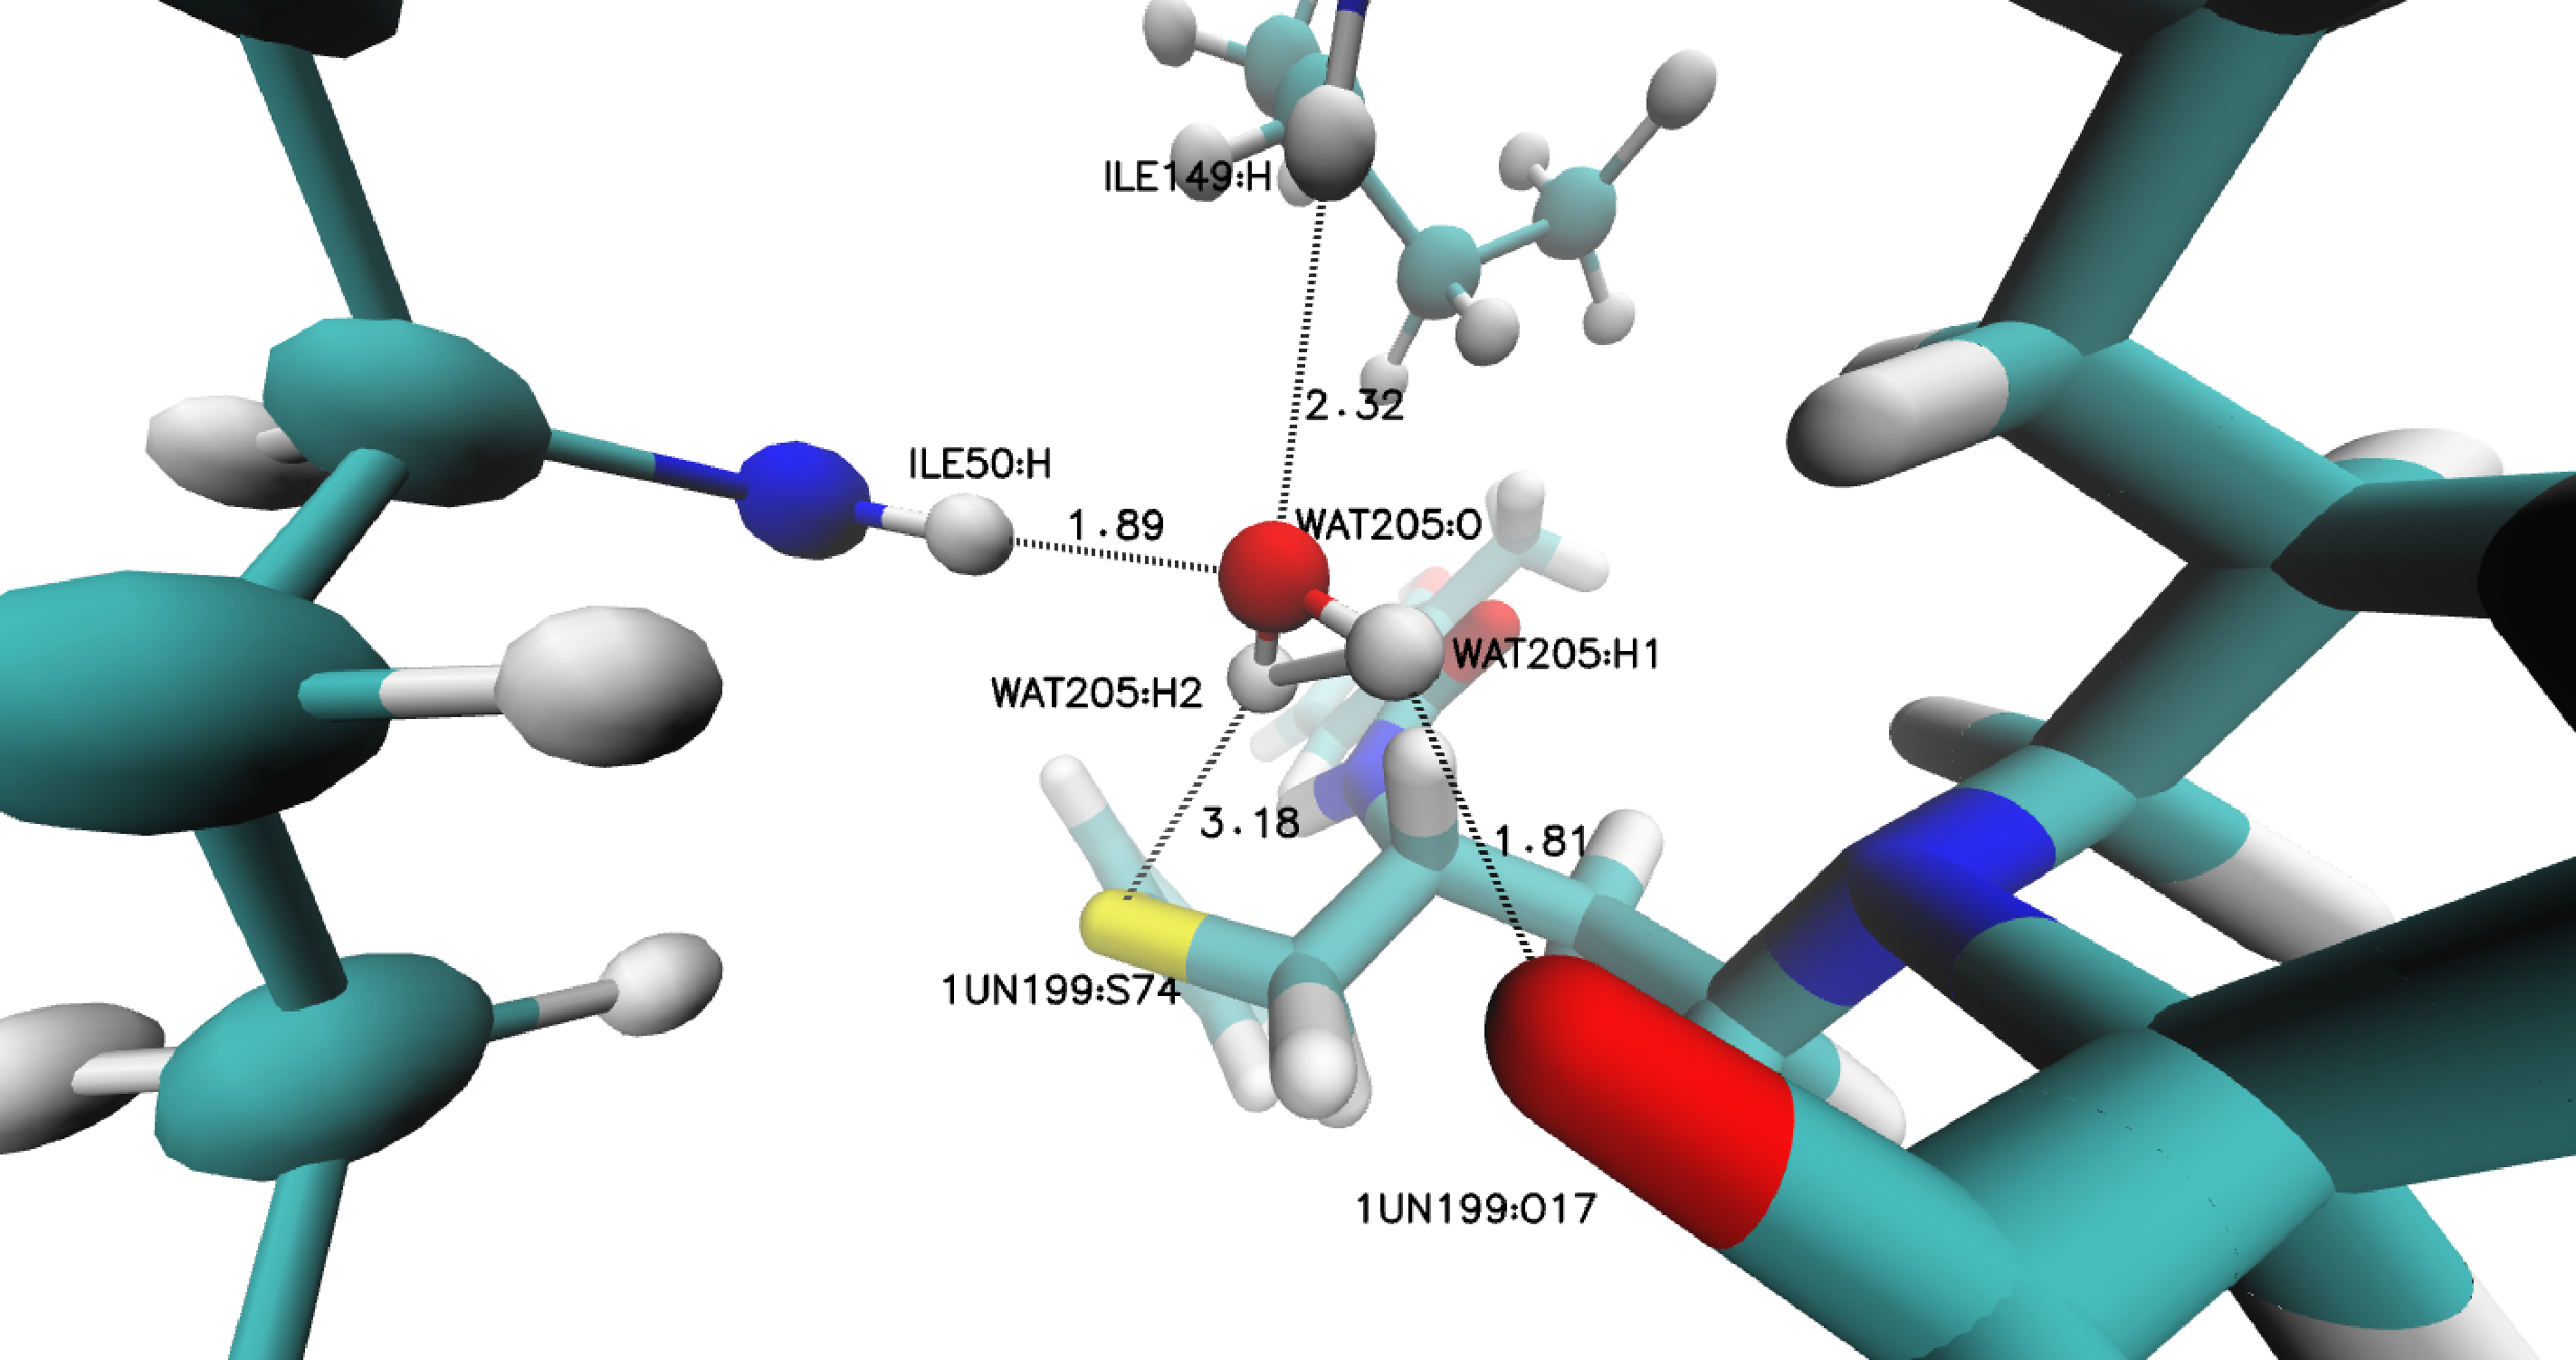
\includegraphics[width=\textwidth]{images/wat205.pdf}
		\caption{}
		\label{fig:an:wat205-vmd}
	\end{subfigure}
	\begin{subfigure}[b]{0.48\textwidth}
		\centering
		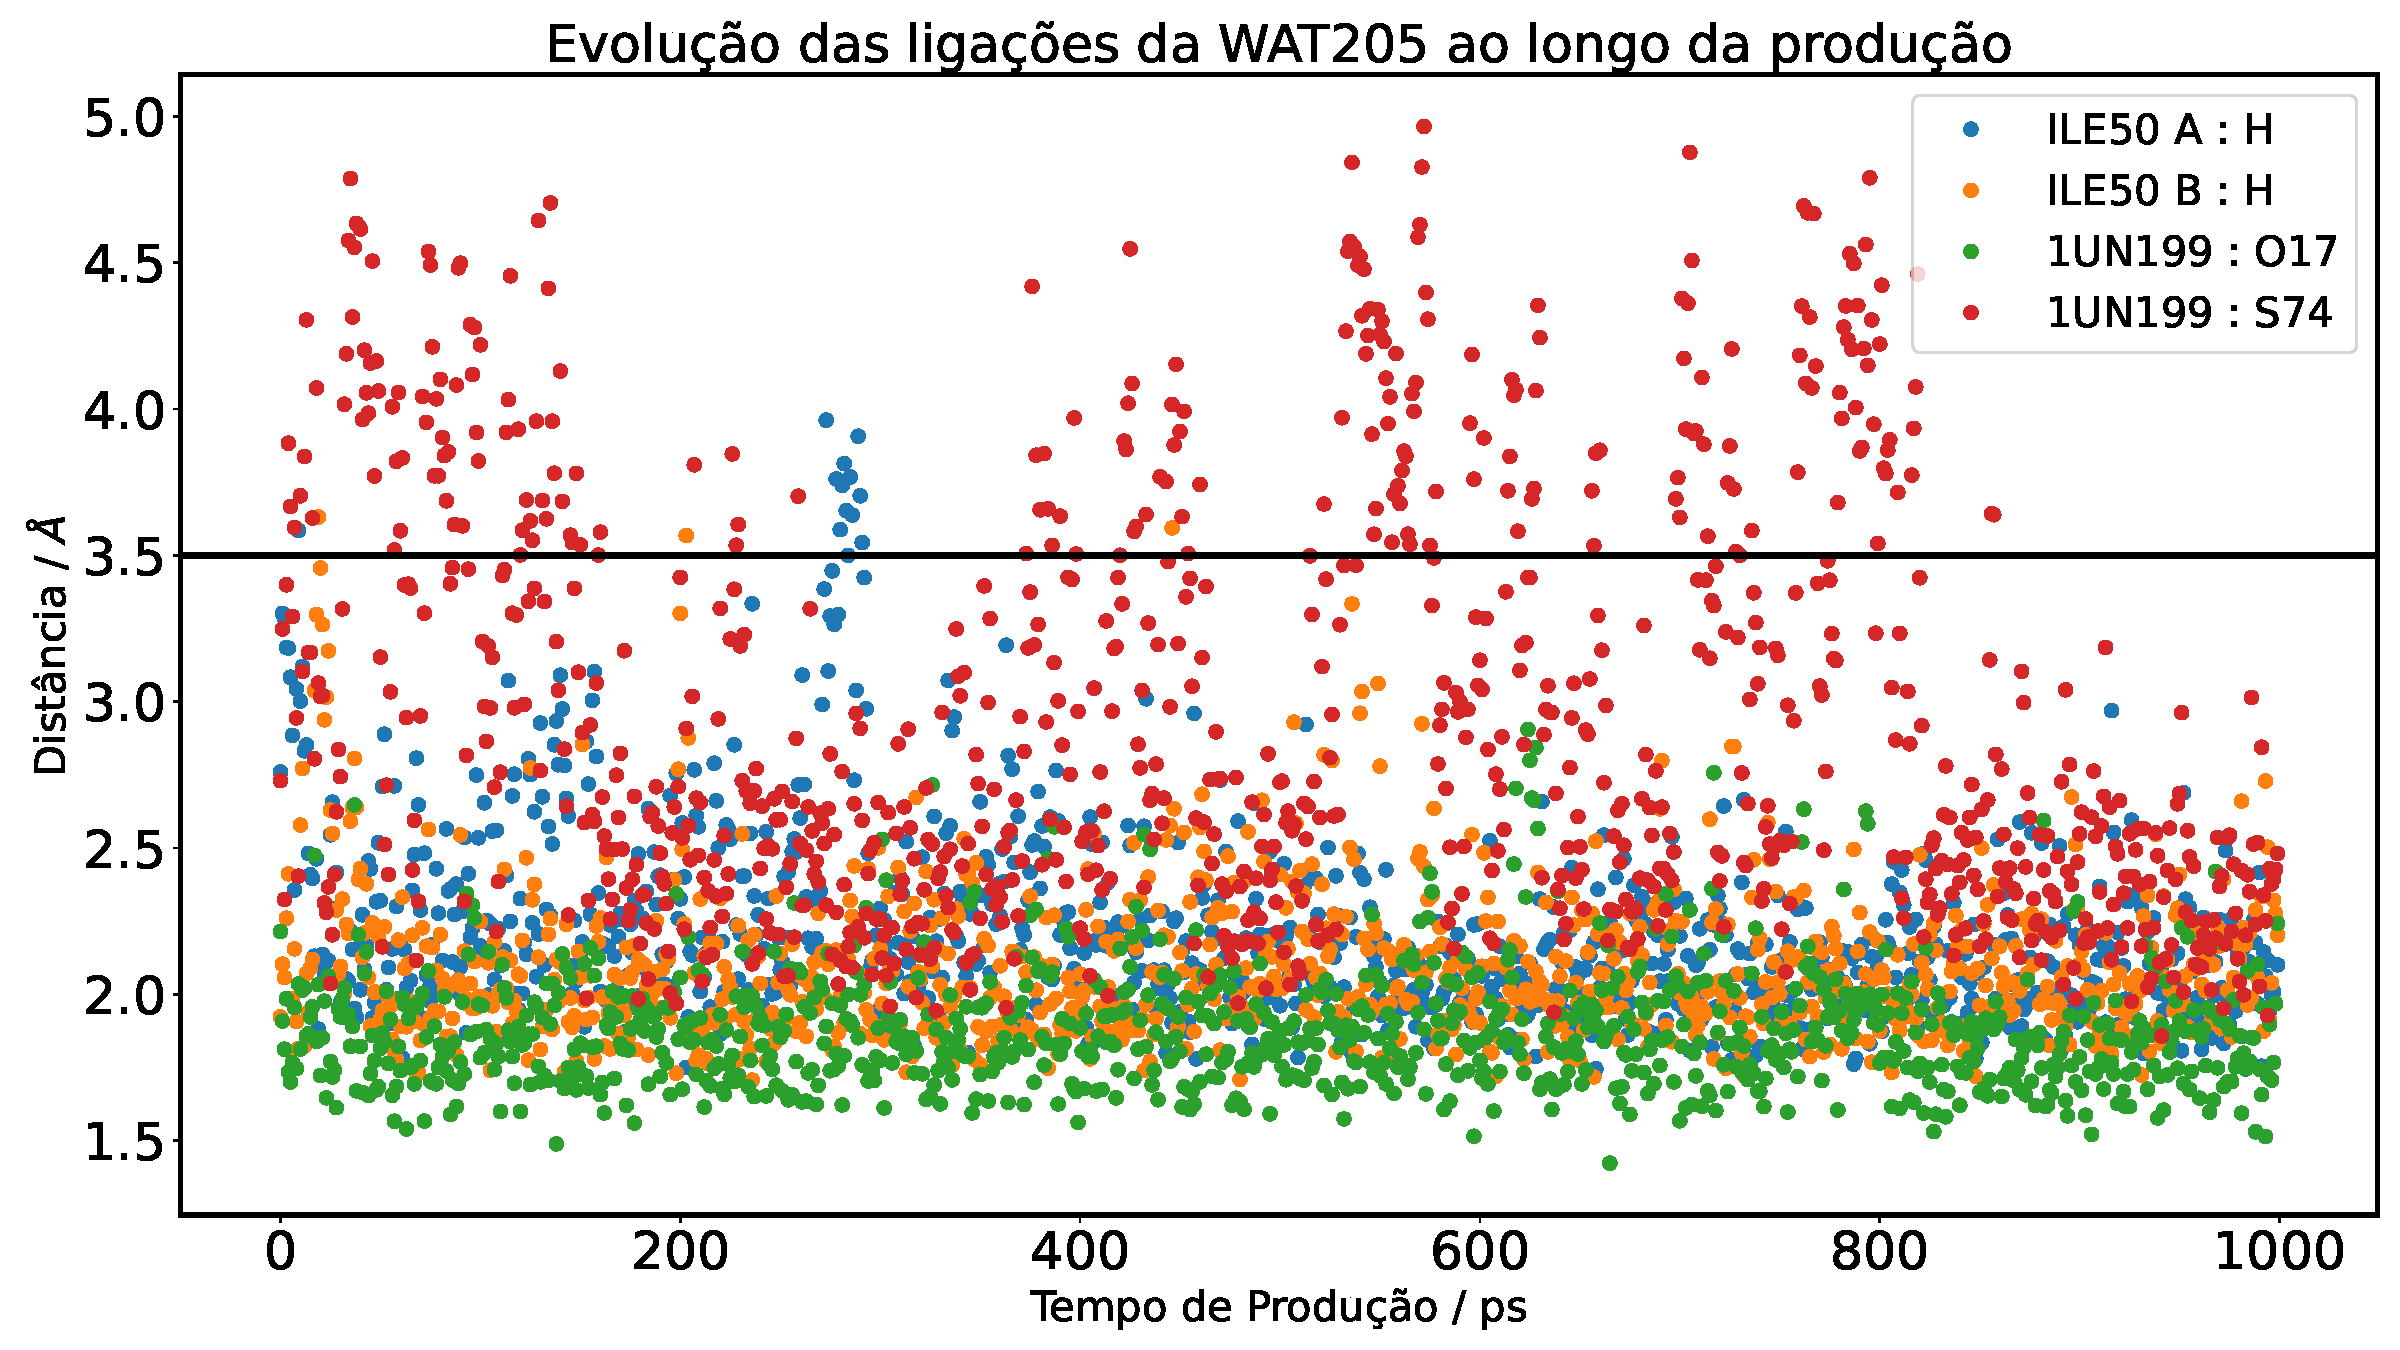
\includegraphics[width=\textwidth]{images/plots-205water.pdf}
		\caption{}
		\label{fig:an:wat205-plot}
	\end{subfigure}
	\caption{\textbf{(a)} Representação das quatro pontes de hidrogénio formadas através da molécula de água catalítica. \textbf{(b)} Gráfico das distâncias (\AA) em função do tempo de produção (ps). As ligações ao inibidor são com os átomos O17 (verde) e S74 (vermelho), e a azul e amarelo estão as ligações com os resíduos ILE50 das cadeias A e B, respetivamente. A linha vertical, $d= 3.5\AA$, assinala o \textit{threshold} a partir do qual não identificamos uma ligação como correspondendo a uma ponte de hidrogénio.}
	\label{fig:an:vars-estruturais}
 	\end{figure}
 
	A \cref{fig:an:wat205-plot} leva-nos a concluir que as pontes de hidrogénio com as ILE50 são muito estáveis, embora haja uma quebra da ligação por volta dos 300 ps, mas que pode ser justificada por uma configuração inicial não otimizada, dado que depois verifica-se que os pontos a azul concentram-se muito mais para distância pequenas. O facto destes resíduos pertencerem à proteína leva-me a concluir que estes são responsáveis pela grande estabilidade da água. 
	
	A água também se encontra fortemente ligada com o O17 do inibidor. No entanto, o S74 é o que quebra a ligação mais frequentemente, mas que acaba por estabilizar abaixo do \textit{treshold} a partir dos 800 ps de produção. Mais tempo de simulação é necessário para determinar se esta relação se mantém ou se surgem pontes de hidrogénio entre átomos diferentes.

\subsection{Propriedades Termodinâmicas e RMSD}
	Como este tipo de sistemas biológicos é estável na natureza, só faz sentido tirar conclusões de um sistema termodinamicamente estável isto é, um sistema cujas propriedades termodinâmicas estejam convergidas. Essas propriedades são: volume, massa, temperatura, pressão e energia. O AMBER foi instruído a imprimir nos ficheiros de output todas as variáveis termodinâmicas que nos interessaram a cada 100 iterações, permitindo-nos construir os gráficos da \cref{fig:an:plots-summary}, onde podemos verificar que todas as variáveis termodinâmicas estudadas convergiram.
	
	Numa discussão do trabalho com o meu colega Pedro Sousa, surgiram-nos dúvidas quanto à viabilidade da fase produção, que supostamente foi teria sido realizada a pressão constante. São evidentes oscilações significativas na pressão do sistema, na ordem das centenas de bar, de iteração para iteração. Consultando o capítulo ``2.5.8 Pressure Regulation'' do \href{https://ambermd.org/doc12/Amber12.pdf}{manual do AMBER}, ficou claro que este tipo de oscilações é esperado do algoritmo, sendo que com o número de iterações a média das pressões irá tender para a pressão objetivo, no nosso caso 1 bar (linha amarela horizontal na \cref{fig:an:plots-summary}). A vermelho foi representada a média móvel de 15 pontos (intervalo de 14 fs) para ilustrar como de facto a média das pressões tende para o valor esperado.
	
	\begin{figure}[h]
	\centering
	\begin{subfigure}[b]{0.48\textwidth}
		\centering
		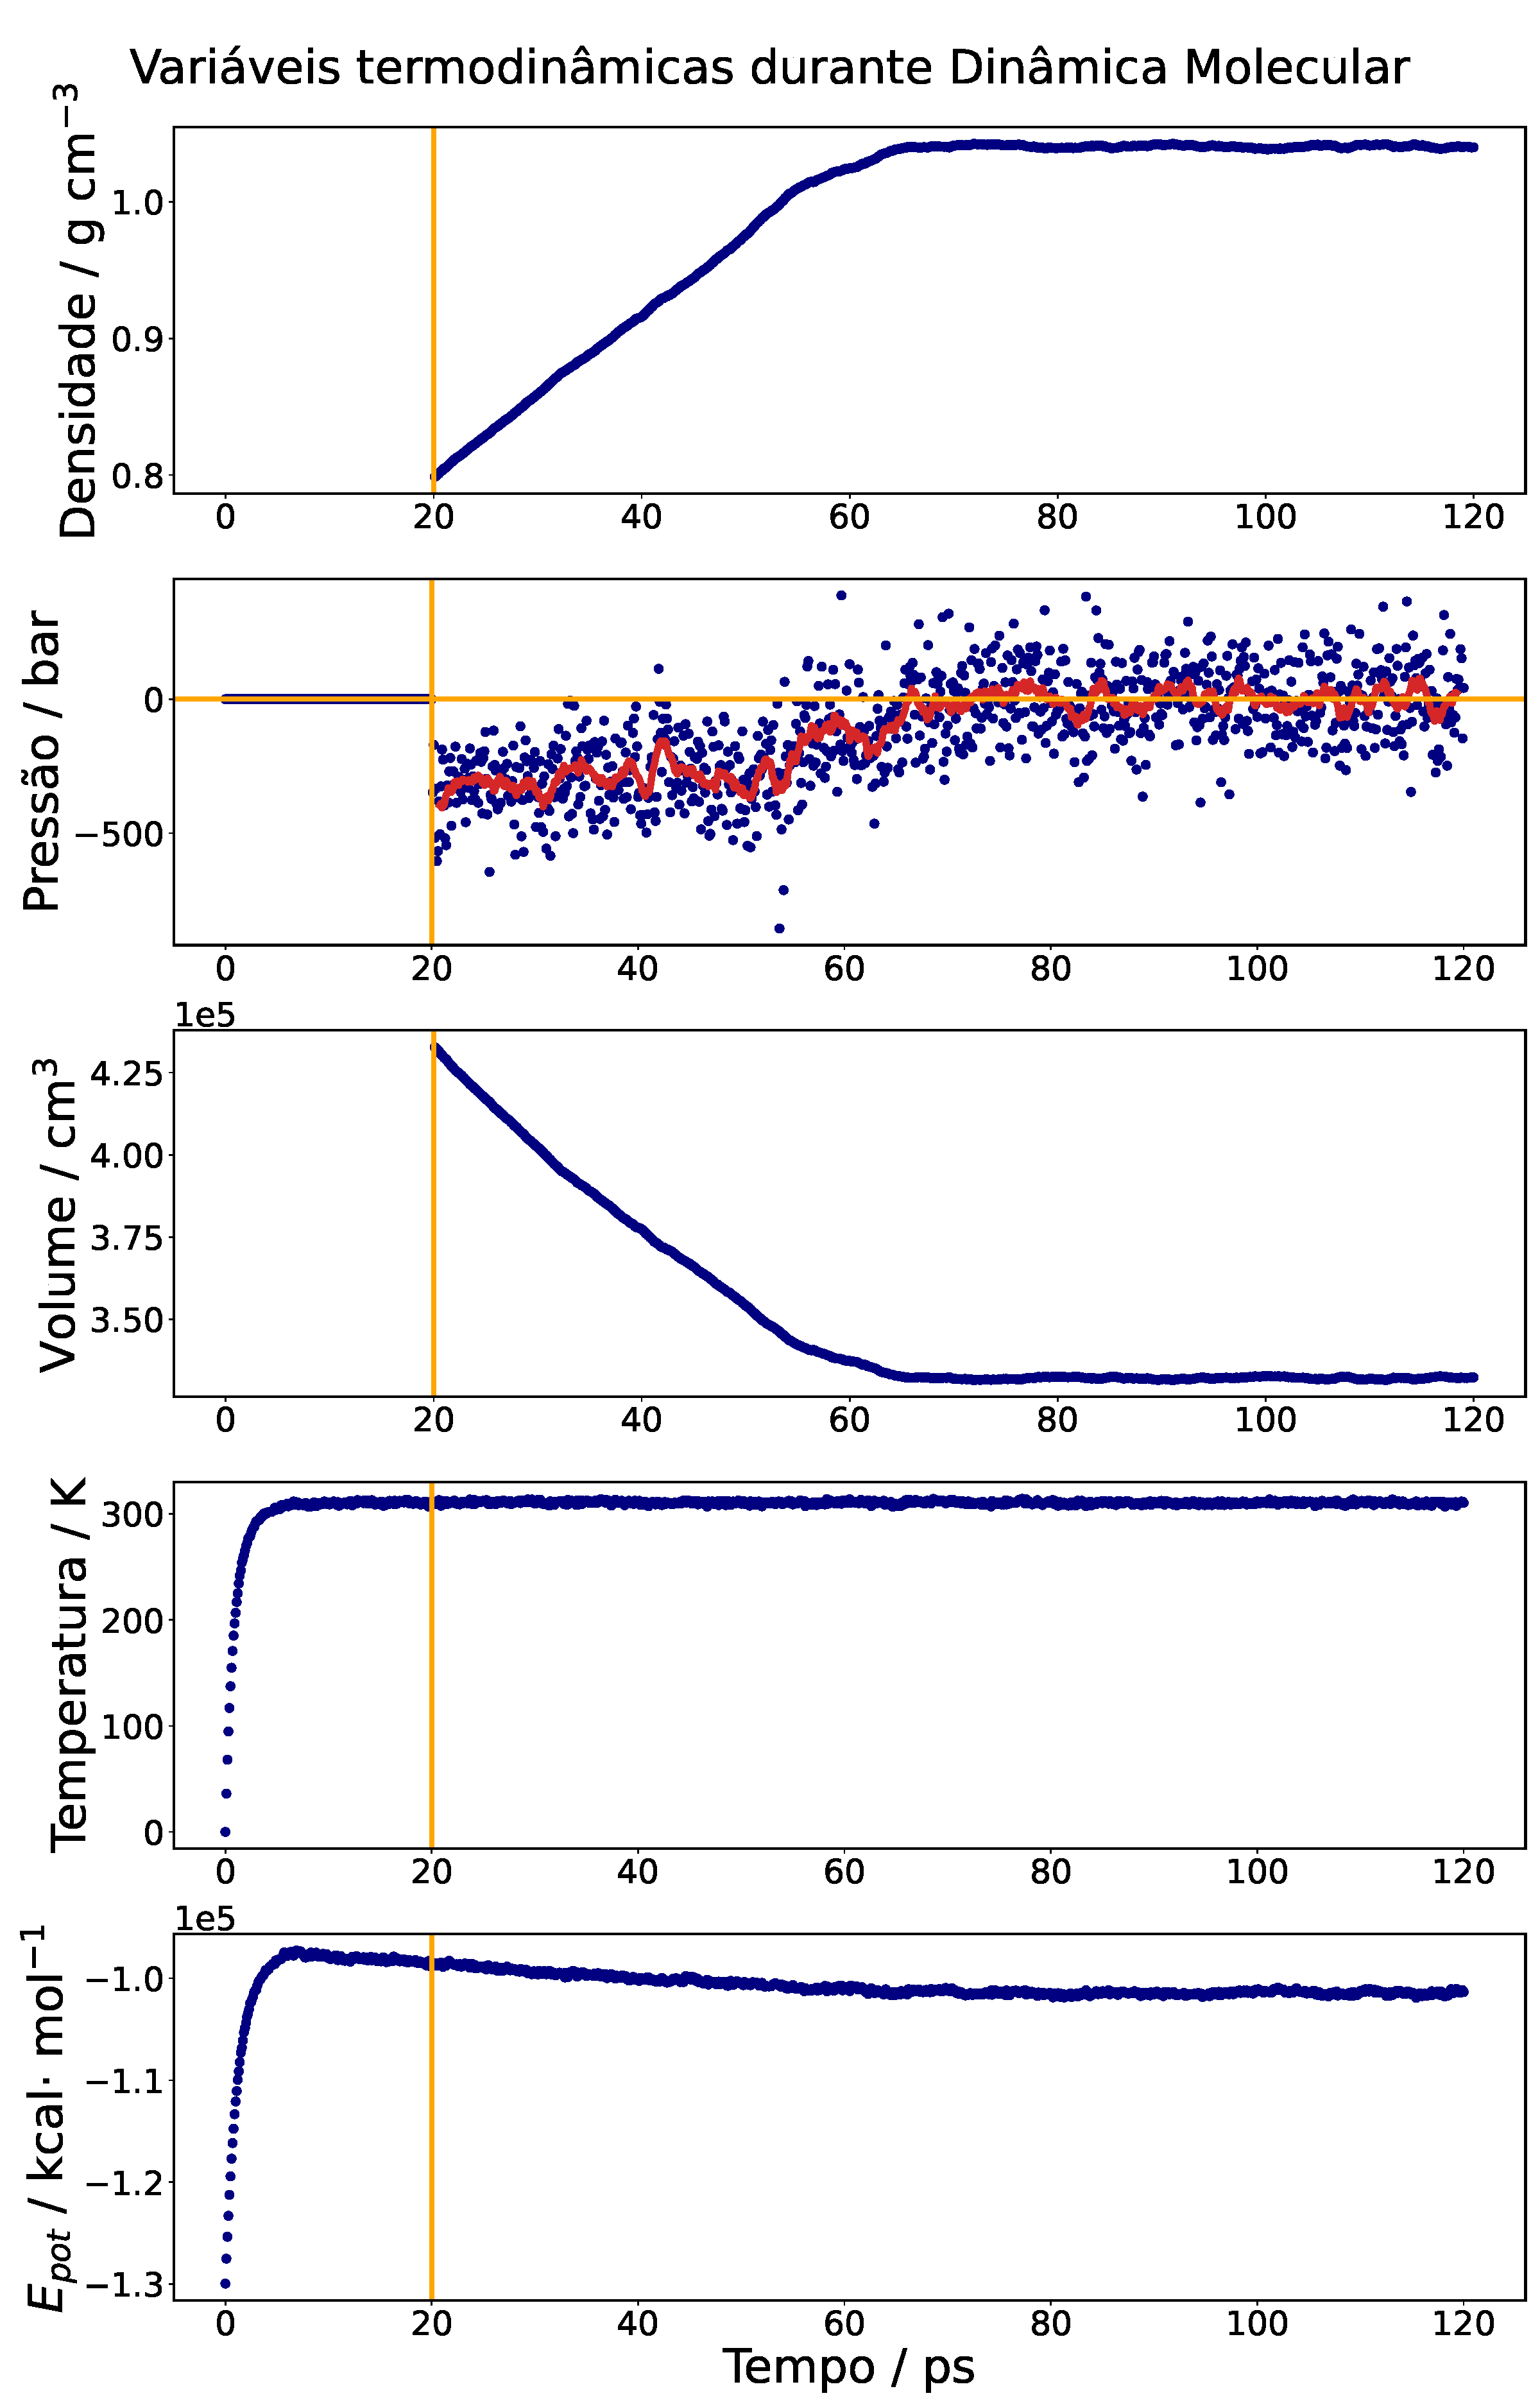
\includegraphics[width=\textwidth]{images/plots-summary.pdf}
		\caption{}
		\label{fig:an:plots-summary}
	\end{subfigure}
	\begin{subfigure}[b]{0.48\textwidth}
		\centering
		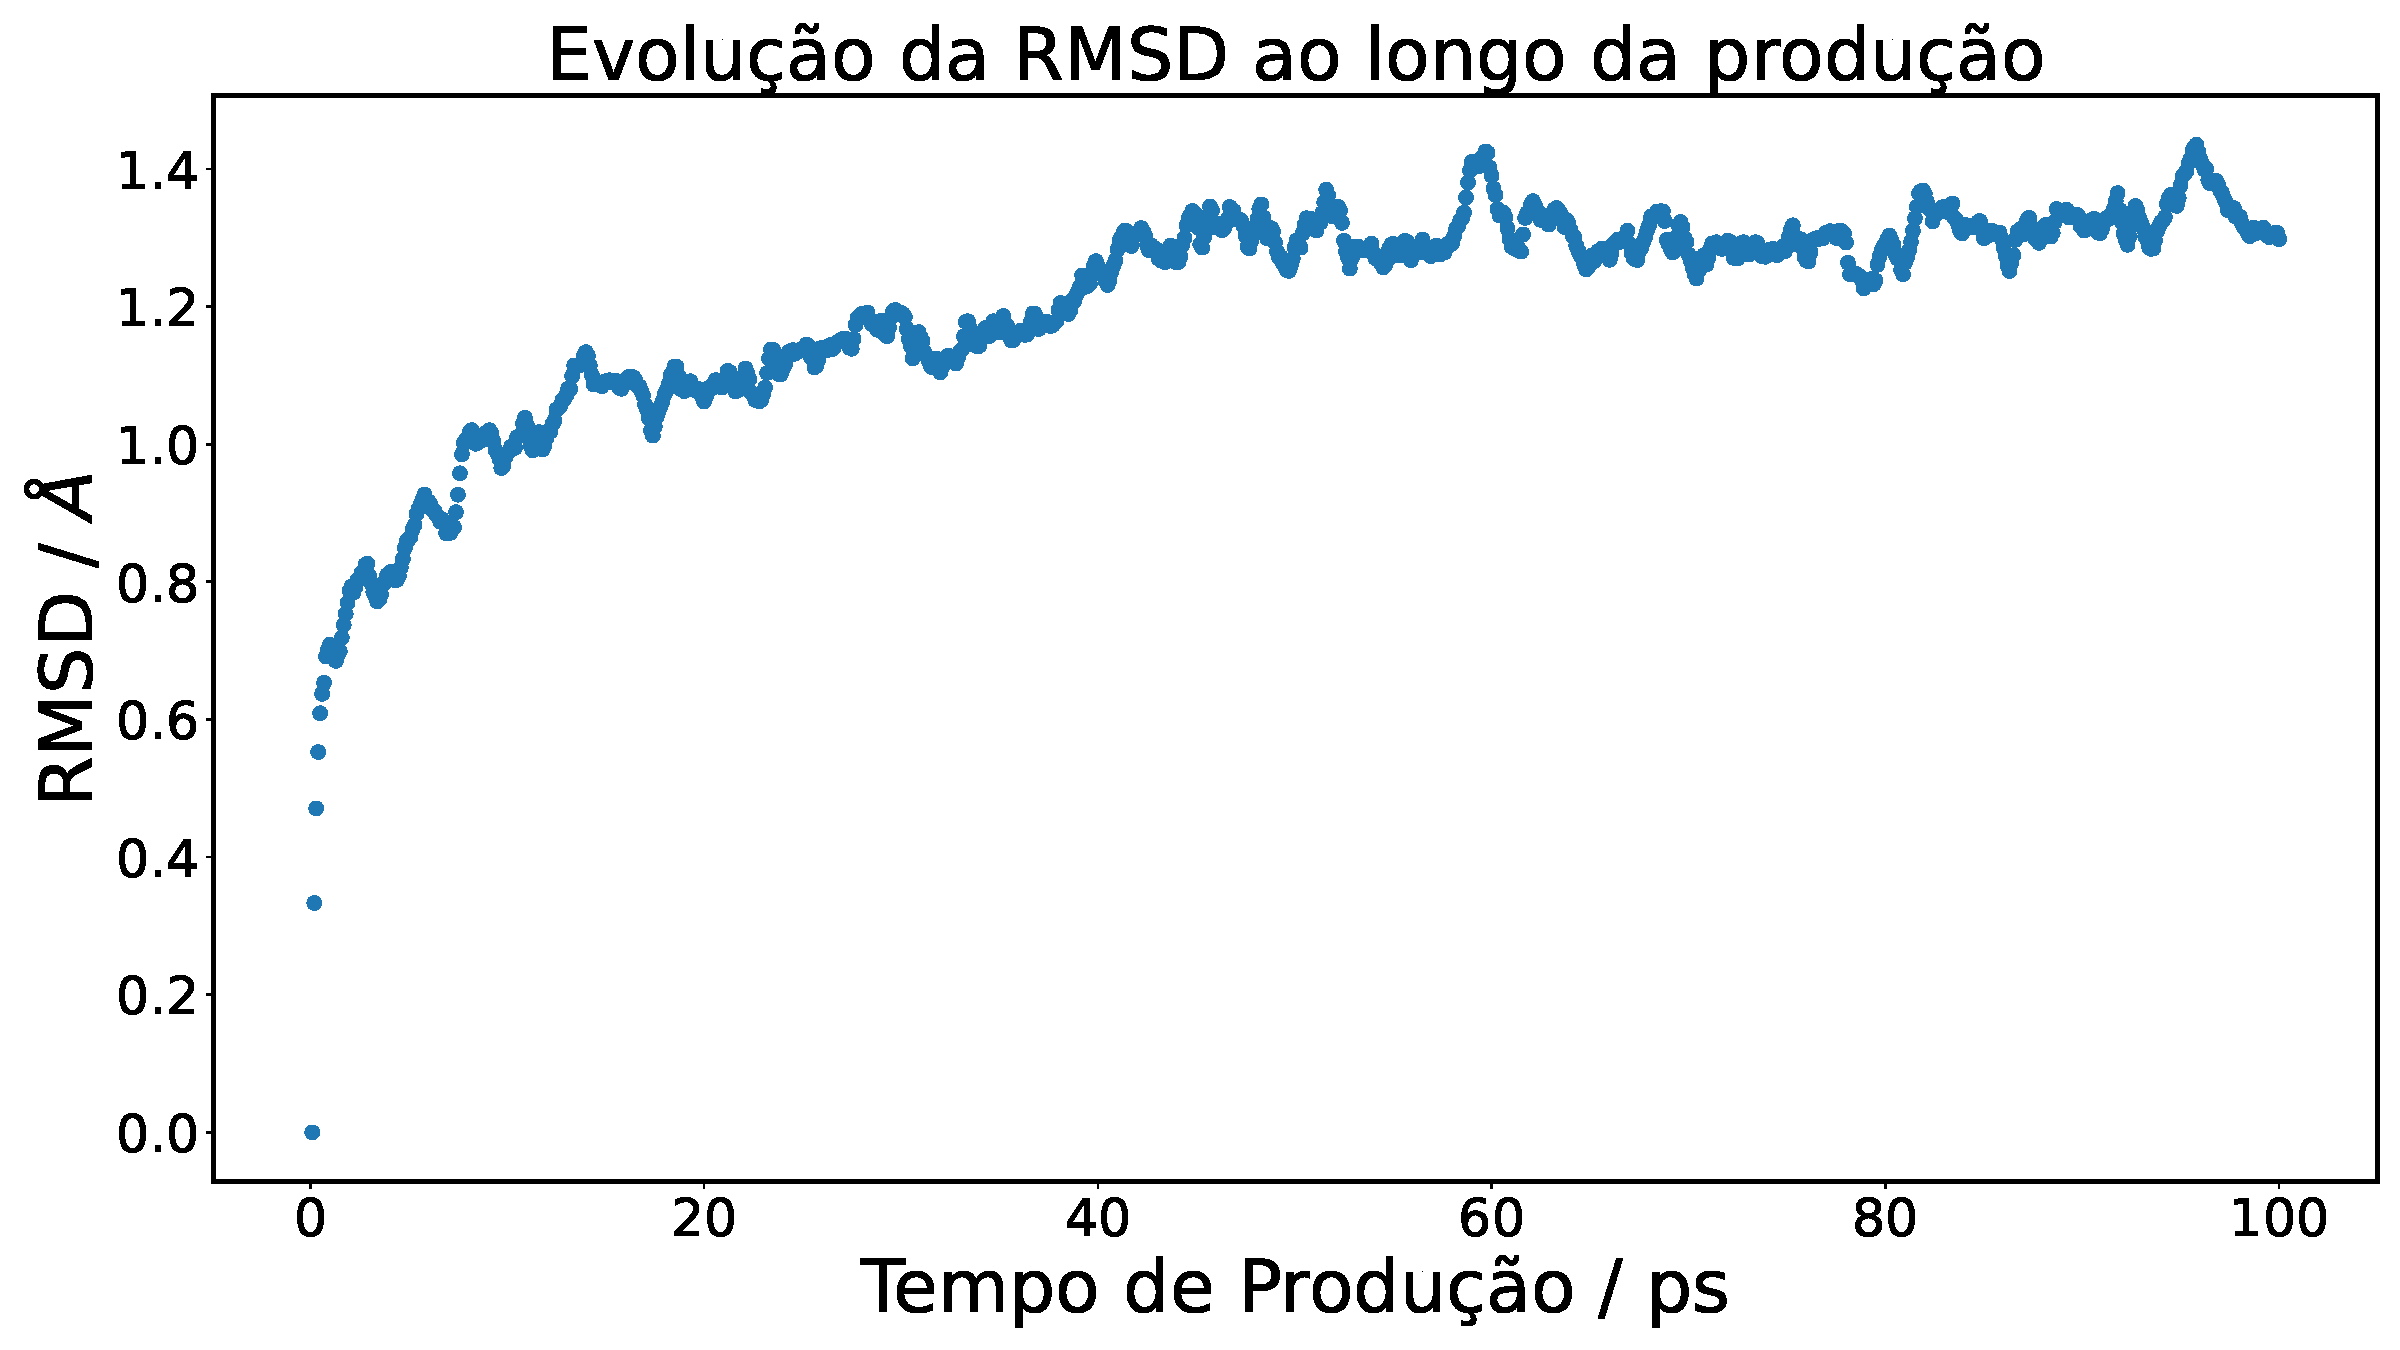
\includegraphics[width=\textwidth]{images/plots-rmsd.pdf}
		\caption{RMSD da fase de produção. \textbf{(a)} Evolução das variáveis termodinâmicas no decorrer das simulações de Dinâmica Molecular. As linhas verticais a laranja indicam $t=20$ ps, o instante de onde de passou da fase de equilibração para a produção. A linha horizontal laranja no gráfico da pressão indica $P = 1$ bar, a pressão objetivo estabelecida para o sistema. Nesse mesmo gráfico está representada a vermelho a média móvel de 15 pontos, correspondente a um intervalo de 14 fs.}
		\label{fig:an:rmsd}
	\end{subfigure}
	\caption{Análise de convergência e estabilidade das simulações de Dinâmica Molecular.}
	\end{figure}
	Depois de verificada a convergência das variáveis termodinâmicas, o próximo gráfico a estudar é o da RMSD - ver \cref{fig:an:rmsd}. Embora a RMSD aparente ter convergido para valores próximos de 1.3 \AA, sabemos que os 120 ps de simulação são extremamente pequenos para sistemas biológicos deste tipo, onde evoluções de dinâmica de molecular de $3-4$ ns são tipicamente realizadas. Se continuássemos a simulação até 12 ns, como os professores fizeram, concluíamos que a estrutura ainda está longe de se encontrar convergida.

\subsection{Função de Distribuição Radial}
	As distribuições radiais constituem um dos métodos mais importantes para a caracterização estrutural das interações entre um soluto e as moléculas do solvente. A ``Radial Distribution Function'' (RDF) entre dois tipos de partículas A e B, $g_{AB}(r)$, representa a densidade de partículas do tipo B à distância $r$ do tipo A.
	
	\begin{figure}[h]
		\begin{subfigure}[l]{0.48\textwidth}
			\centering
			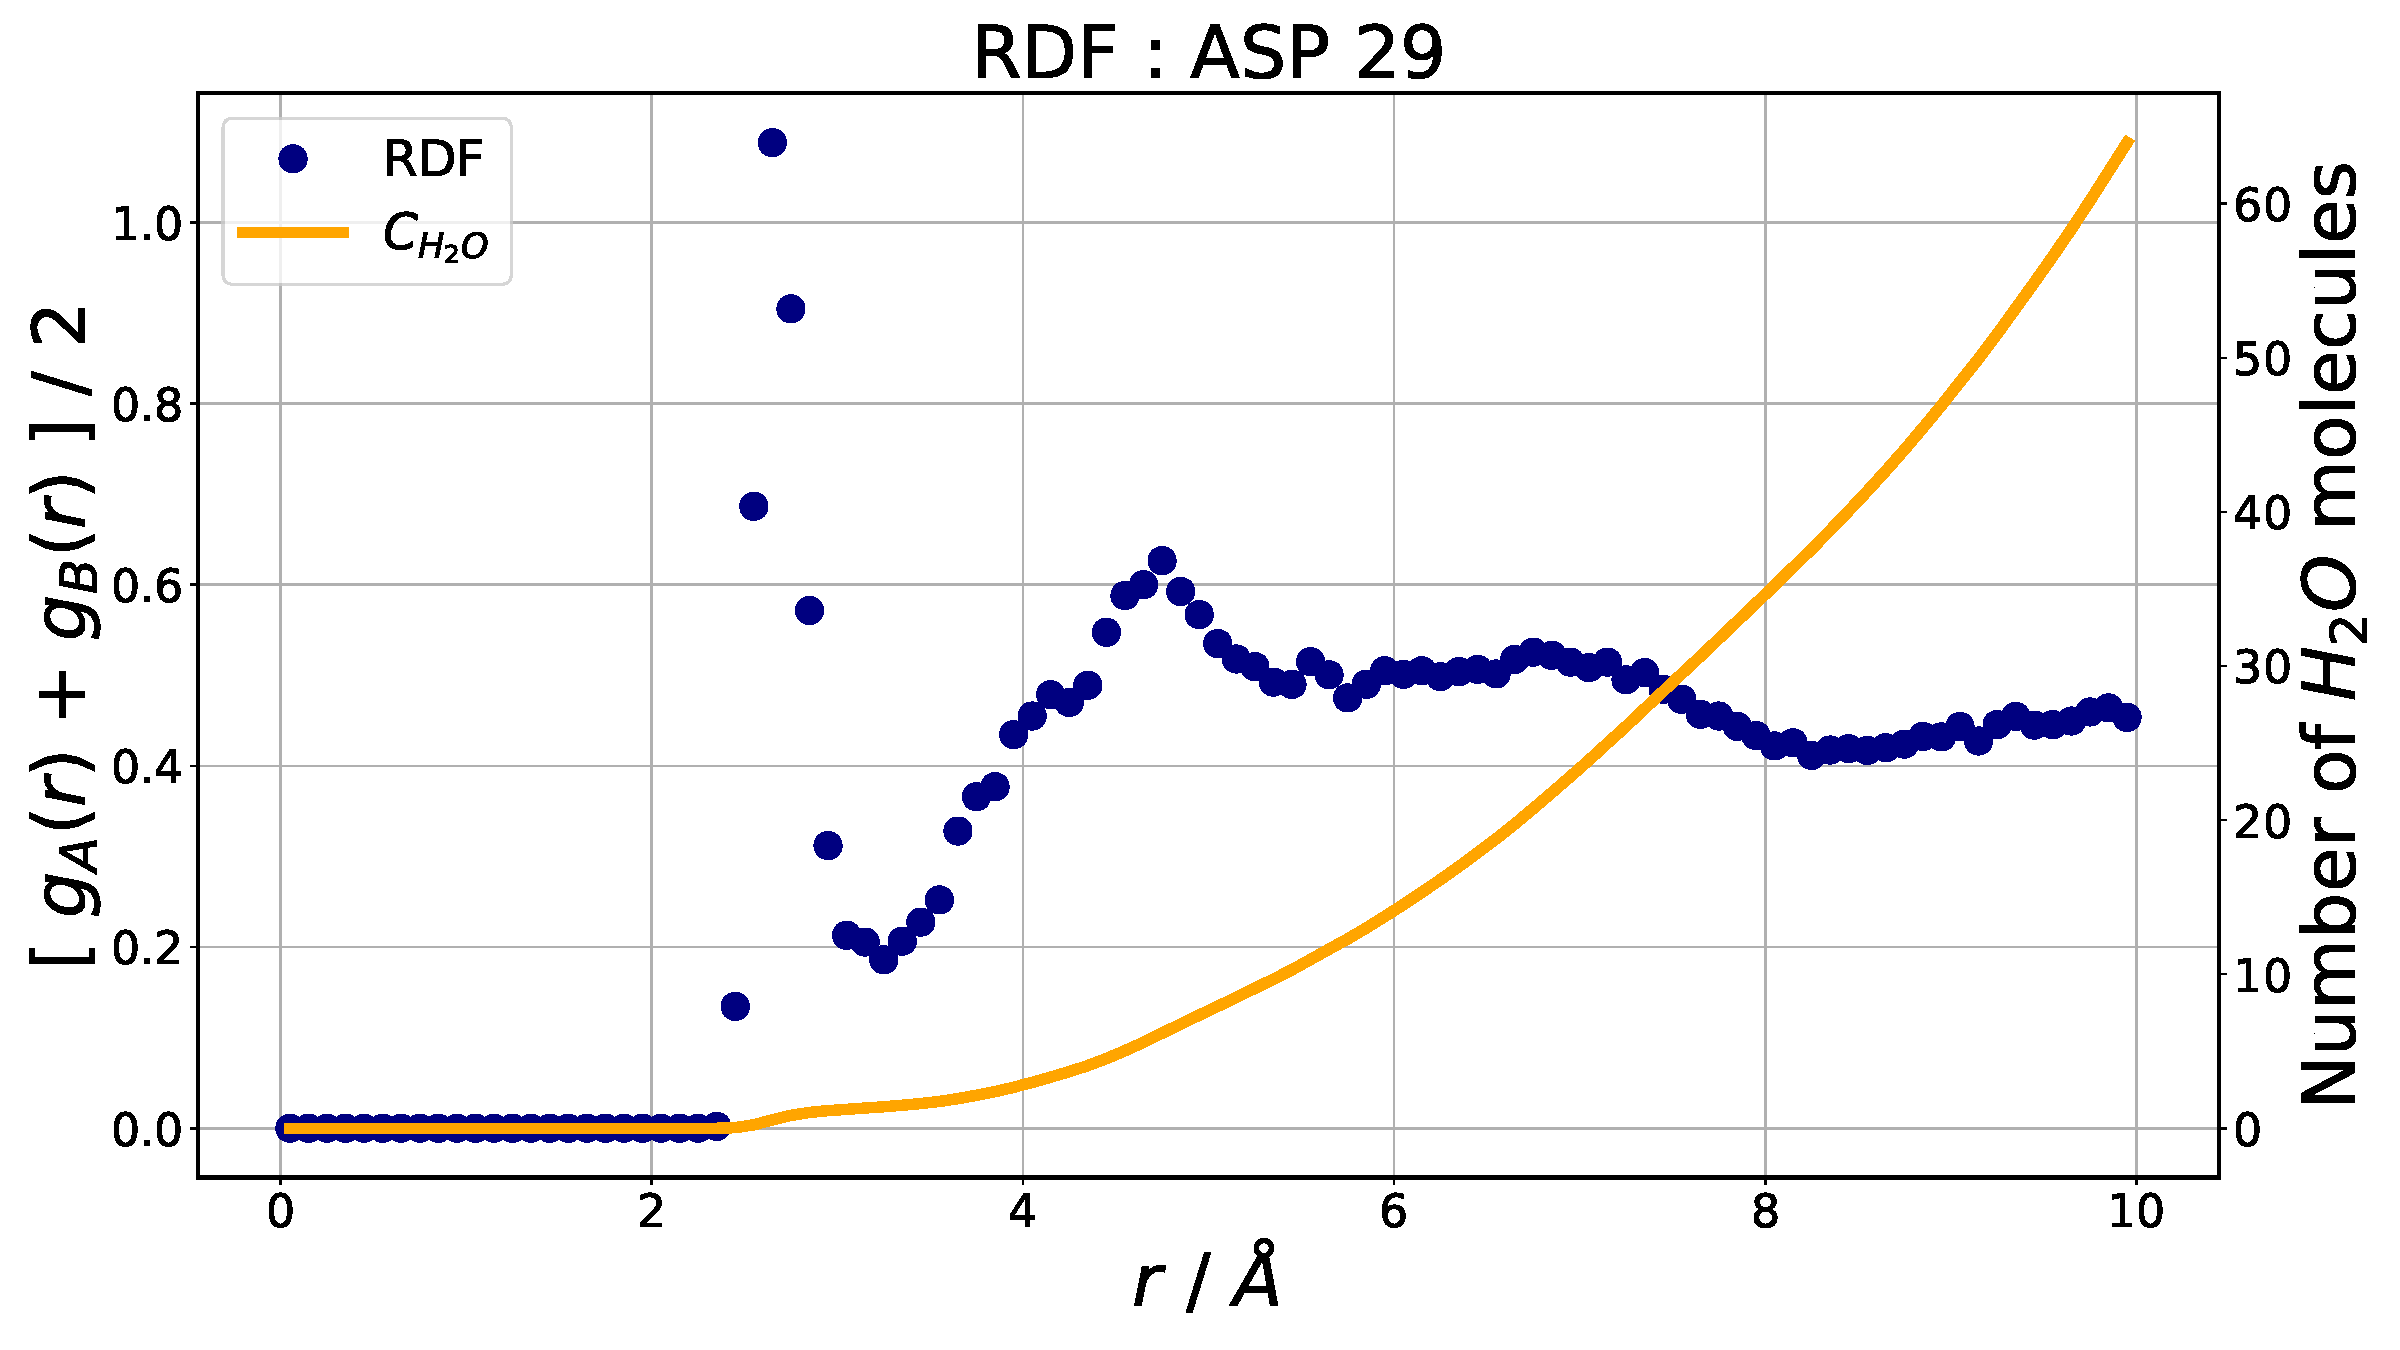
\includegraphics[width=\textwidth]{images/plots-rdf-ASP29.pdf}
			\caption{}
			\label{fig:an:rdf-asp29}
		\end{subfigure}
		\begin{subfigure}[r]{0.48\textwidth}
			\centering
			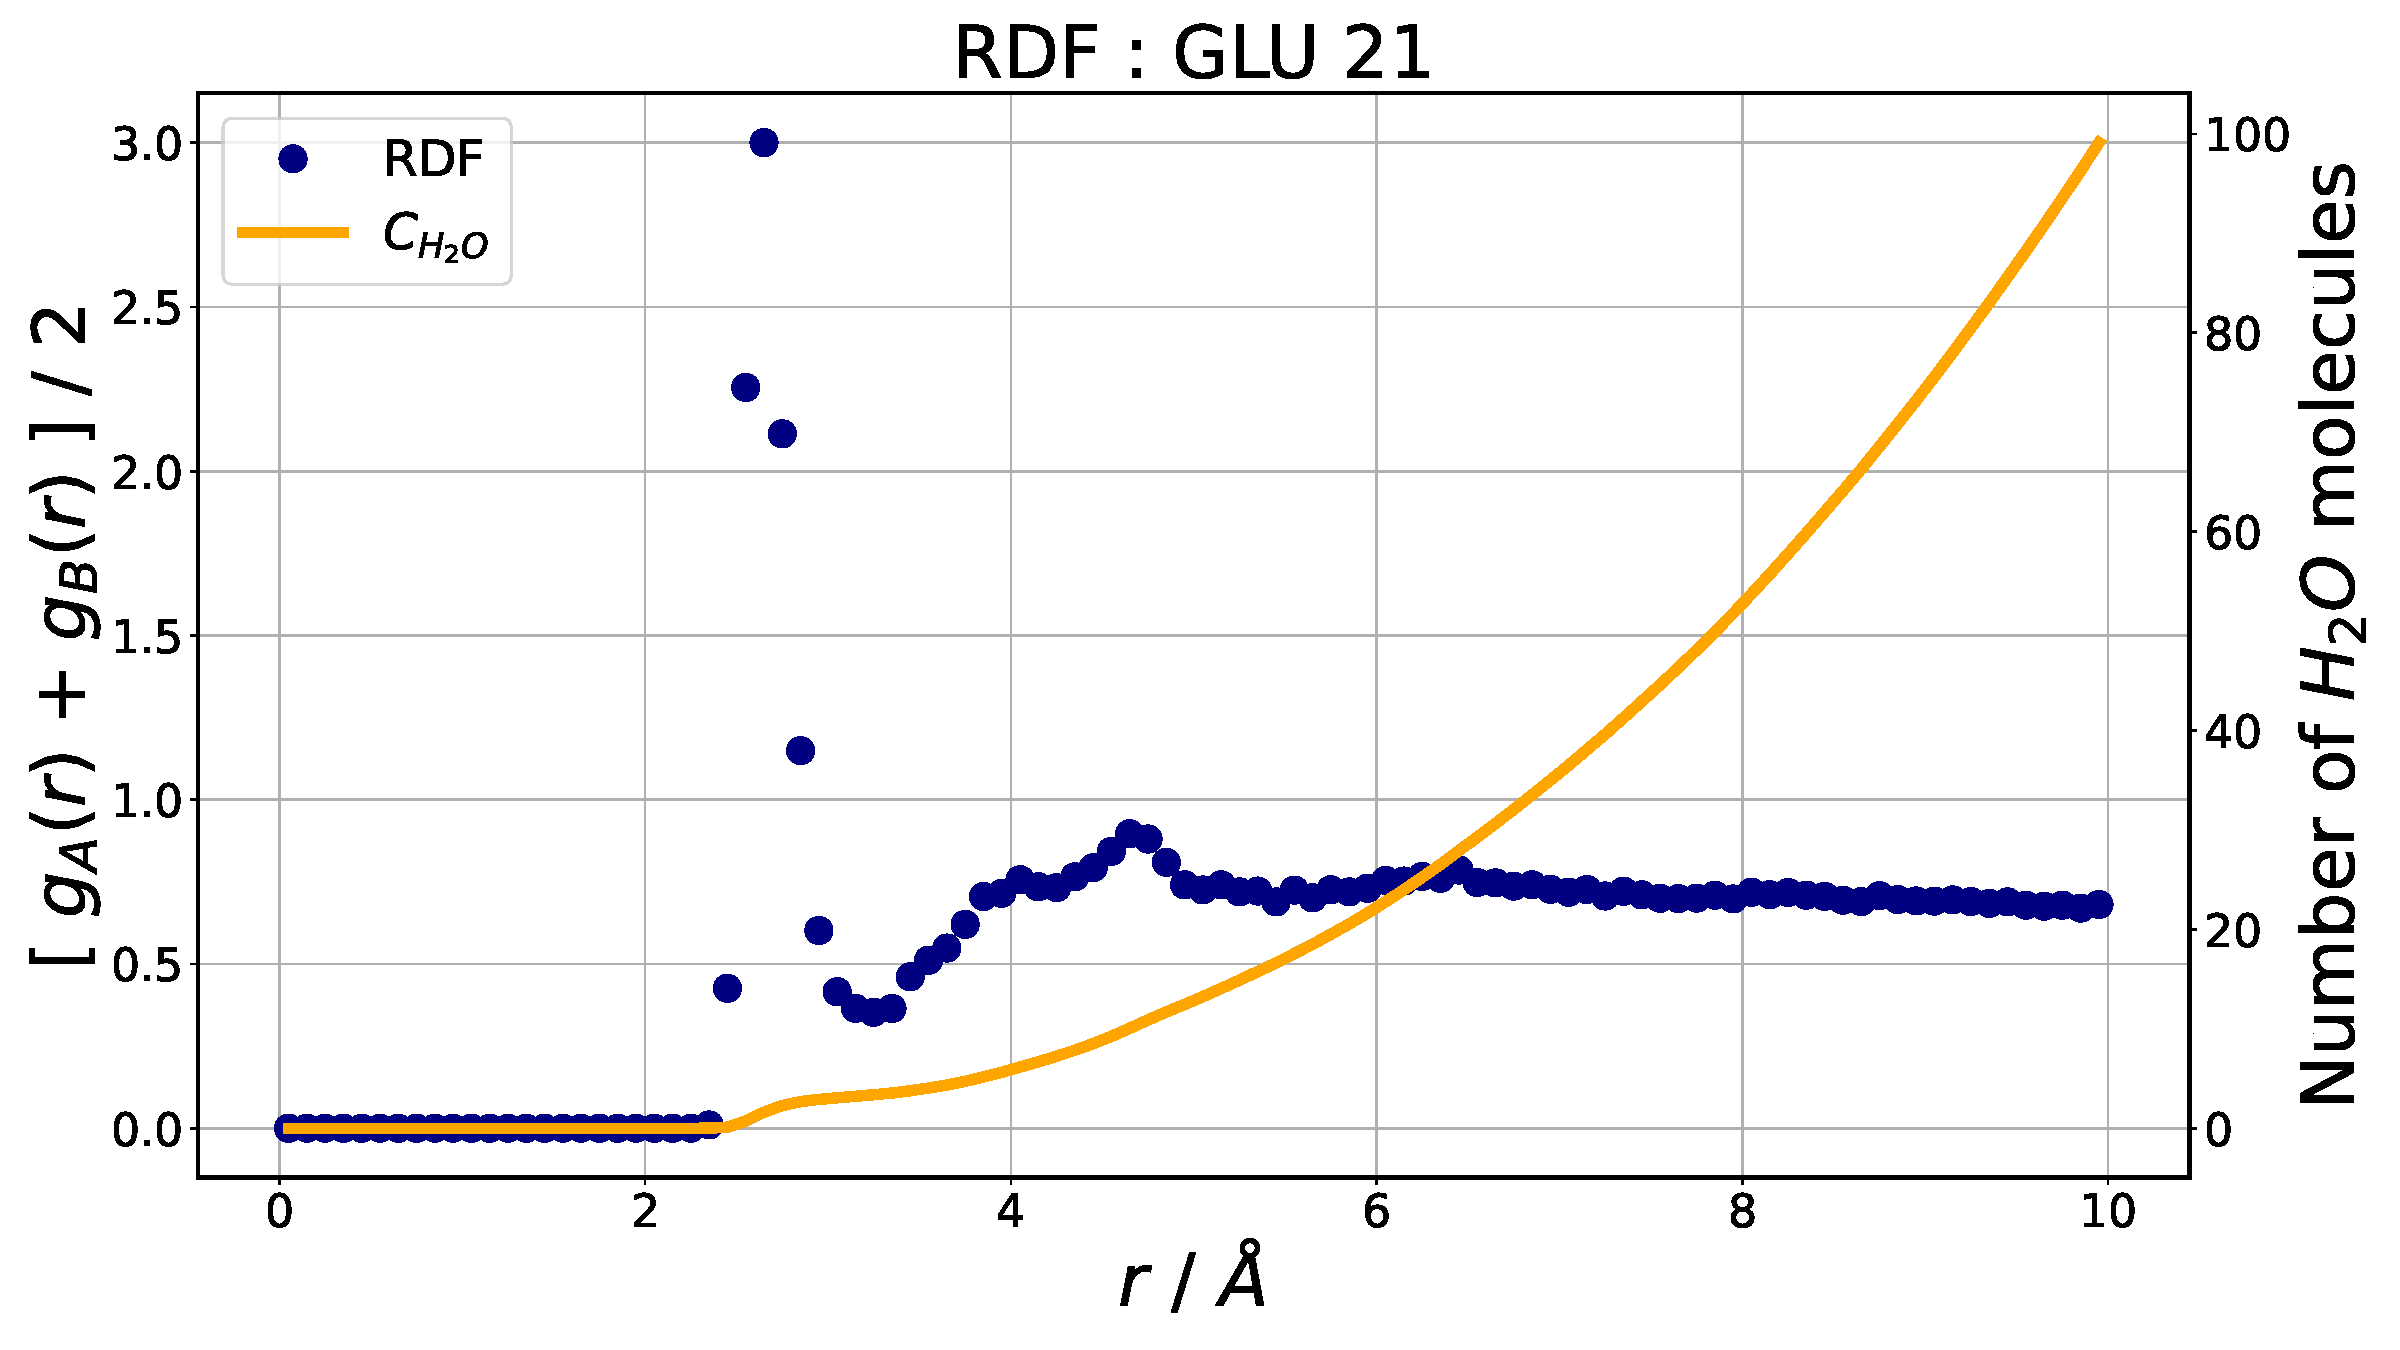
\includegraphics[width=\textwidth]{images/plots-rdf-GLU21.pdf}
			\caption{}
			\label{fig:an:rdf-glu21}
		\end{subfigure}
		\centering
		\begin{subfigure}[b]{0.6\textwidth}
			\centering
			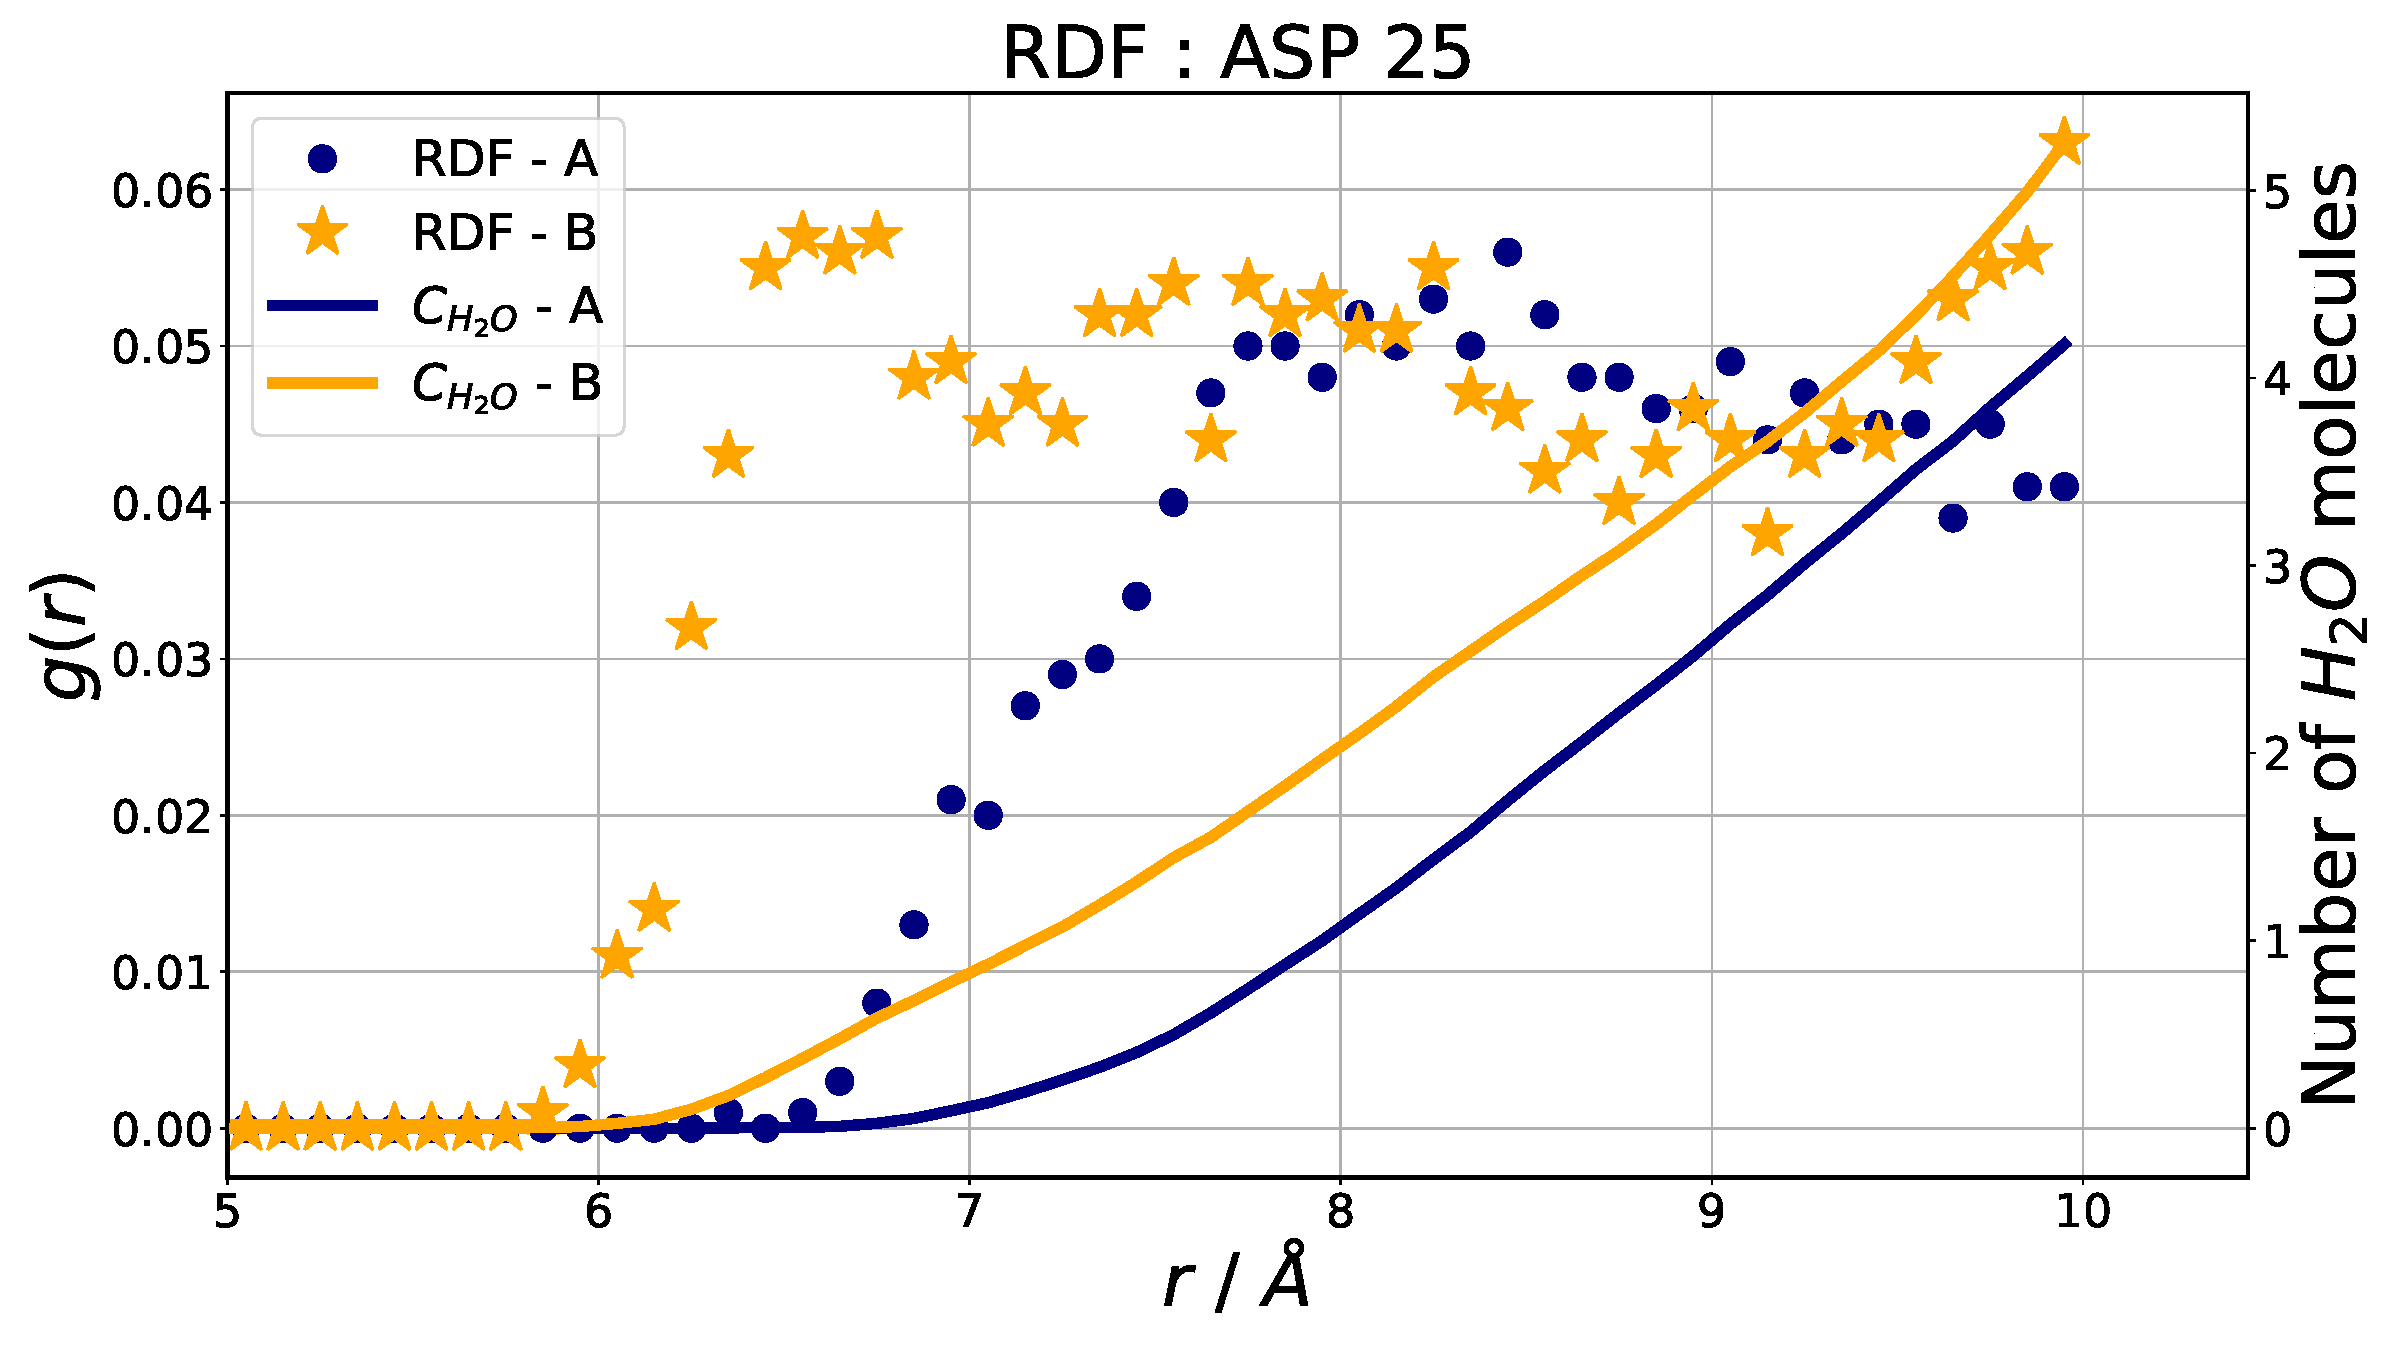
\includegraphics[width=\textwidth]{images/plots-rdf-ASP25.pdf}
			\caption{}
			\label{fig:an:rdf-asp25}
		\end{subfigure}
		\caption{Funções de Distribuição Radial (pontos) e número de moléculas de água (linhas a cheio) em função da distância aos resíduos ASP29:OD$^{*}$ \textbf{(a)}, GLU21:OE$^{*}$ \textbf{(b)}, e ASP25:OD$^{*}$ \textbf{(c)}. Os dois primeiros gráficos foram obtidos através da média dos resultados para as cadeias A e B. Por outro lado, os dados para o ASP25 estão distinguidos por cadeia, uma vez que o ASP da cadeia B está protonado nesta estrutura.}
		\label{fig:an:rdf-all}
	\end{figure}

	Estas funções foram determinadas usando o comando \verb|ptraj| do AMBER para os resíduos ASP25, ASP29 e GLU21 da proteína. O solvente analisado foi a água que envolve a proteína. Os resultados destes cálculos estão representados na \cref{fig:an:rdf-all} assim como a contagem de moléculas de água analisadas à medida que nos afastamos dos átomos de referência. Os princípios físicos que governam os vários picos observados podem ser consultados em \cite{boydElectronDensityPartitioning1977,politzerSeparationCoreValence1976}, sendo que cada mínimo indica o fim de uma esfera de solvatação.
	
	Na \cref{fig:an:rdf-asp25} conseguimos distinguir três esferas de solvatação para a cadeia B, presentes a $r\approx 7.1, 8.0$ e $9.0\AA$. Não consigo identificar com clareza numa destas esferas para o o ASP da cadeia A. Note-se que as RDFs começam a ganhar amplitude ligeiramente antes dos 6\AA. Por outro lado, as distribuições para os resíduos ASP29 e GLU21 ganham amplitude por volta dos 2.2 \AA\ e possuem duas esferas de solvatação a $r\approx 3.5$ e $r \approx5.5 \AA$, embora esta última seja pouco evidente.
	
	Note-se que a \cref{fig:an:rdf-asp25} revela claras assimetrias entre os dois ácidos aspárticos, evidenciando o quanto a protonação do resíduo influencia a química dos processos na vizinhança desta zona da proteína. As distâncias elevadas observadas neste gráfico revelam que a água catalítica se encontra demasiado afastada destes resíduos para se poderem estabelecer pontes de hidrogénio entre eles. Um resultado curioso é que a primeira esfera de solvatação do ASP25 da cadeia B contém apenas uma molécula de água, a segunda contém duas, e a terceira três, todas separadas por aproximadamente 1\AA. Em contrapartida, para as GLU21 e ASP29, a primeira molécula de água surge a 2.85 e 2.65 \AA\ dos respetivos átomos de referência.
	
	Outro resultado interessante desta análise é o valor para o qual vemos que as densidades convergem para $r>9\AA$. A convergência dá-se porque quanto mais nos afastamos do átomo de referência, menor a influência terão esses átomos sobre estas camadas exteriores e menor será a contribuição da densidade das camadas interiores para o cálculo médio da densidade, ou seja, aproximamo-nos da homogeneidade. No entanto, seria de esperar uma tendência para 1 (densidade da água) e não $\approx0.5$, como se verifica. Isto acontece porque aproximadamente metade do volume contido nas cascas esféricas para o cálculo da RDF é preenchido pela protease, que não contribui para a função densidade do solvente. Se expandíssemos a análise para raios maiores acabaríamos por ver o patamar esperado para a RDF. Porém, esse estudo não faria sentido porque nas nossas simulações só foram consideradas interações num raio de $10 \AA$ de cada átomo.
	
\subsection{Ligações de Hidrogénio}
	O \verb|ptraj| foi novamente utilizado, desta vez para determinar os comprimentos ($d$) e ângulos ($\theta$) de ligação de todas as pontes de hidrogénio presentes no sistema. Na \cref{fig:an:hbonds-table} é apresentado um \textit{print} do \textit{output} destes cálculos com as cinco principais pontes de hidrogénio, onde o valor de ocupação indica a percentagem de \textit{snapshots} do sistema em que a ligação em questão cumpria as condições para se qualificar como ponte de hidrogénio, um indicador da estabilidade da ligação, tendo-se detetado um total de 202 ligações deste tipo.
	
	Para tentar encontrar os valores de $d$ e $\theta$ que conferem maior estabilidade às ligações construiu-se o gráfico da \cref{fig:an:hbonds-plot}. Embora esta análise seja muito primitiva e superficial, os valores de $d$ mais estáveis parecem estar em torno dos $2.8 - 2.9$ \AA, e os de $\theta$ mais próximos do intervalo $160 - 165 ^{\circ}$.
	
	Uma análise mais detalha passaria por distinguir as ligações por aceitadores e dadores, para podermos isolar as variações de $d$ e $\theta$ das variações de vizinhança em que ocorrem.
	
	\begin{figure}[h]
		\centering
		\includegraphics[width=0.9\textwidth]{images/table-hbonds.png}
		\caption{Tabela com as cinco pontes de hidrogénio mais estáveis do sistema ao londo dos 120 ps de DM. Podemos facilmente identificar os átomos dadores e aceitadores de cada uma. Os valores entre ``()'' correspondem à incerteza da medição em questão.}
		\label{fig:an:hbonds-table}
	\end{figure}
	\begin{figure}[h]
		\centering
		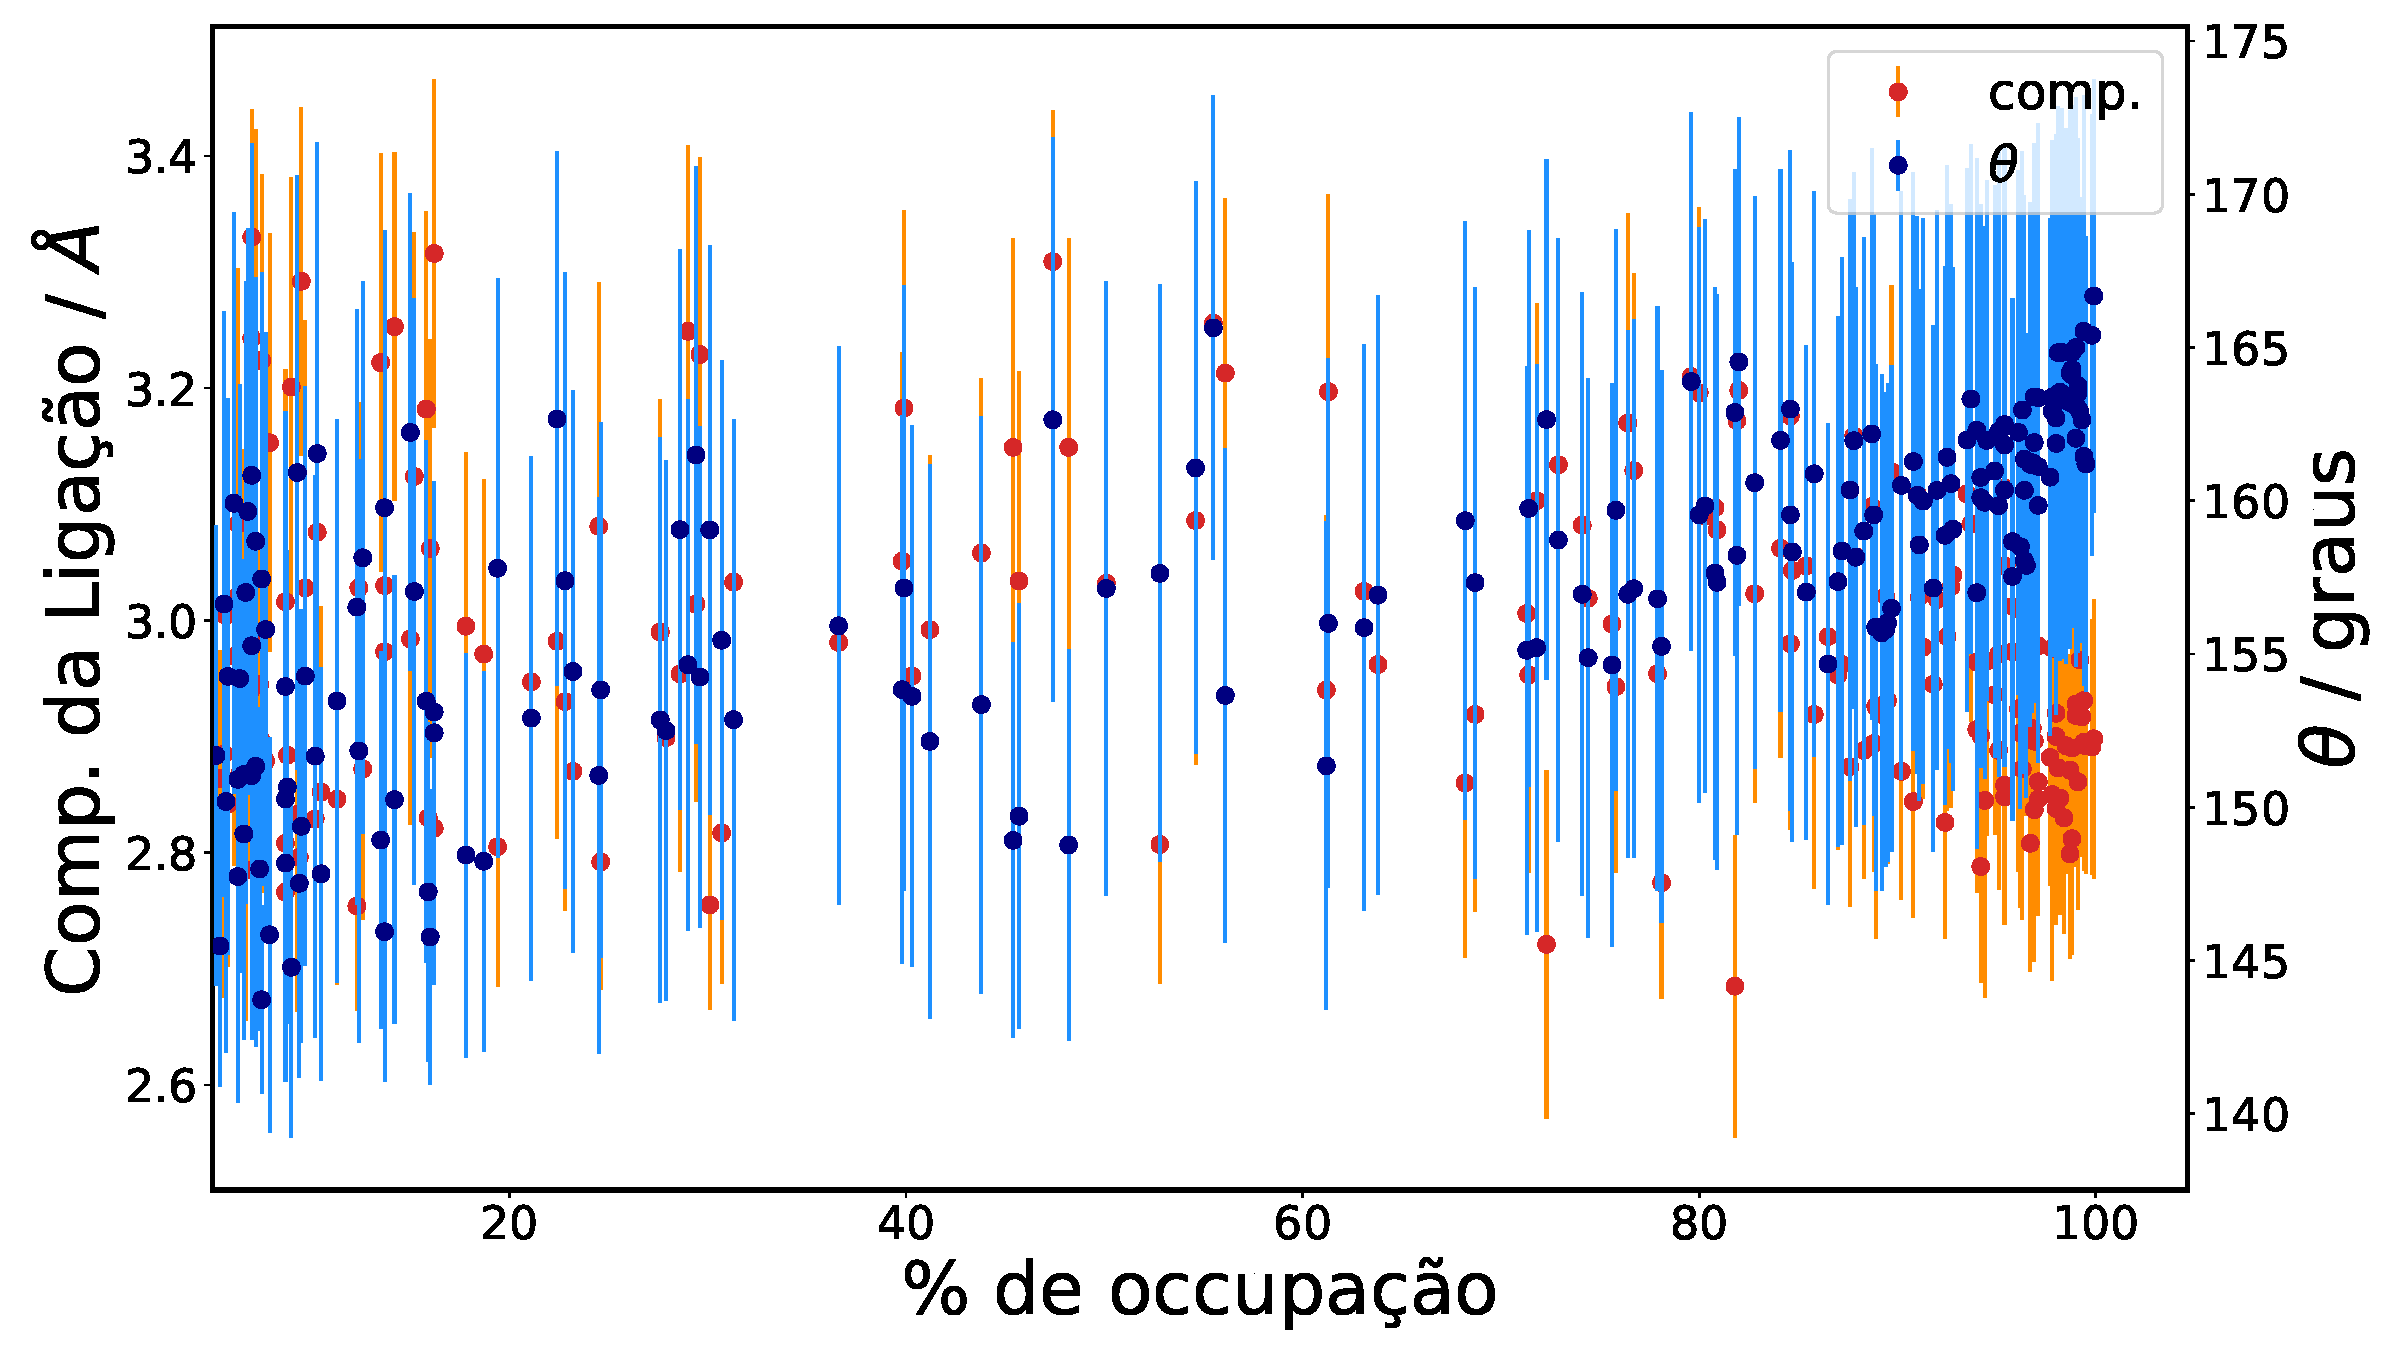
\includegraphics[width=0.7\textwidth]{images/plots-hbonds-linear.pdf}
		\caption{Representação dos comprimentos e ângulos de ligação para as 202 pontes de H estudadas, a vermelho e azul, respetivamente. As barras de erro estão representadas a tons mais leves das respetivas cores.}
		\label{fig:an:hbonds-plot}	
	\end{figure}


\subsection{Cálculo de Distâncias e Ângulos}
	Na Sec. (\ref{sec:variacoes-estruturais}) foi apresentado uma breve análise dos comprimentos de ligação das pontes de hidrogénio da água catalítica usando o VMD - ver \cref{fig:an:vars-estruturais}. O VMD também é capaz de determinar ângulos de ligação e diedros com a mesma facilidade. Estas grandezas podem ter muito interesse conforme o tipo de análise em que estamos interessados. No entanto, o método é pouco autonomizável, por ser necessário selecionar manualmente os átomos numa interface gráfica. É neste contexto que entra mais uma vez o \verb|ptraj|, que nos permite determinar as grandezas referidas com grande facilidade.
	
	Na \cref{fig:an:dists-vmd} estão representadas as ligações que o inibidor forma com os OD* dos resíduos ASP25 (cadeia A)  e ASH124 (cadeia B). Estes dois resíduos são aqueles que estão implícitos quando menciono ``os resíduos ASP25''. Os comprimentos de ligação foram representados graficamente na \cref{fig:an:dists-plot}, onde estão devidamente assinaladas a média e o desvio padrão para cada uma das ligações.
	
	\begin{figure}[h]
		\begin{subfigure}[b]{0.34\textwidth}
			\centering
			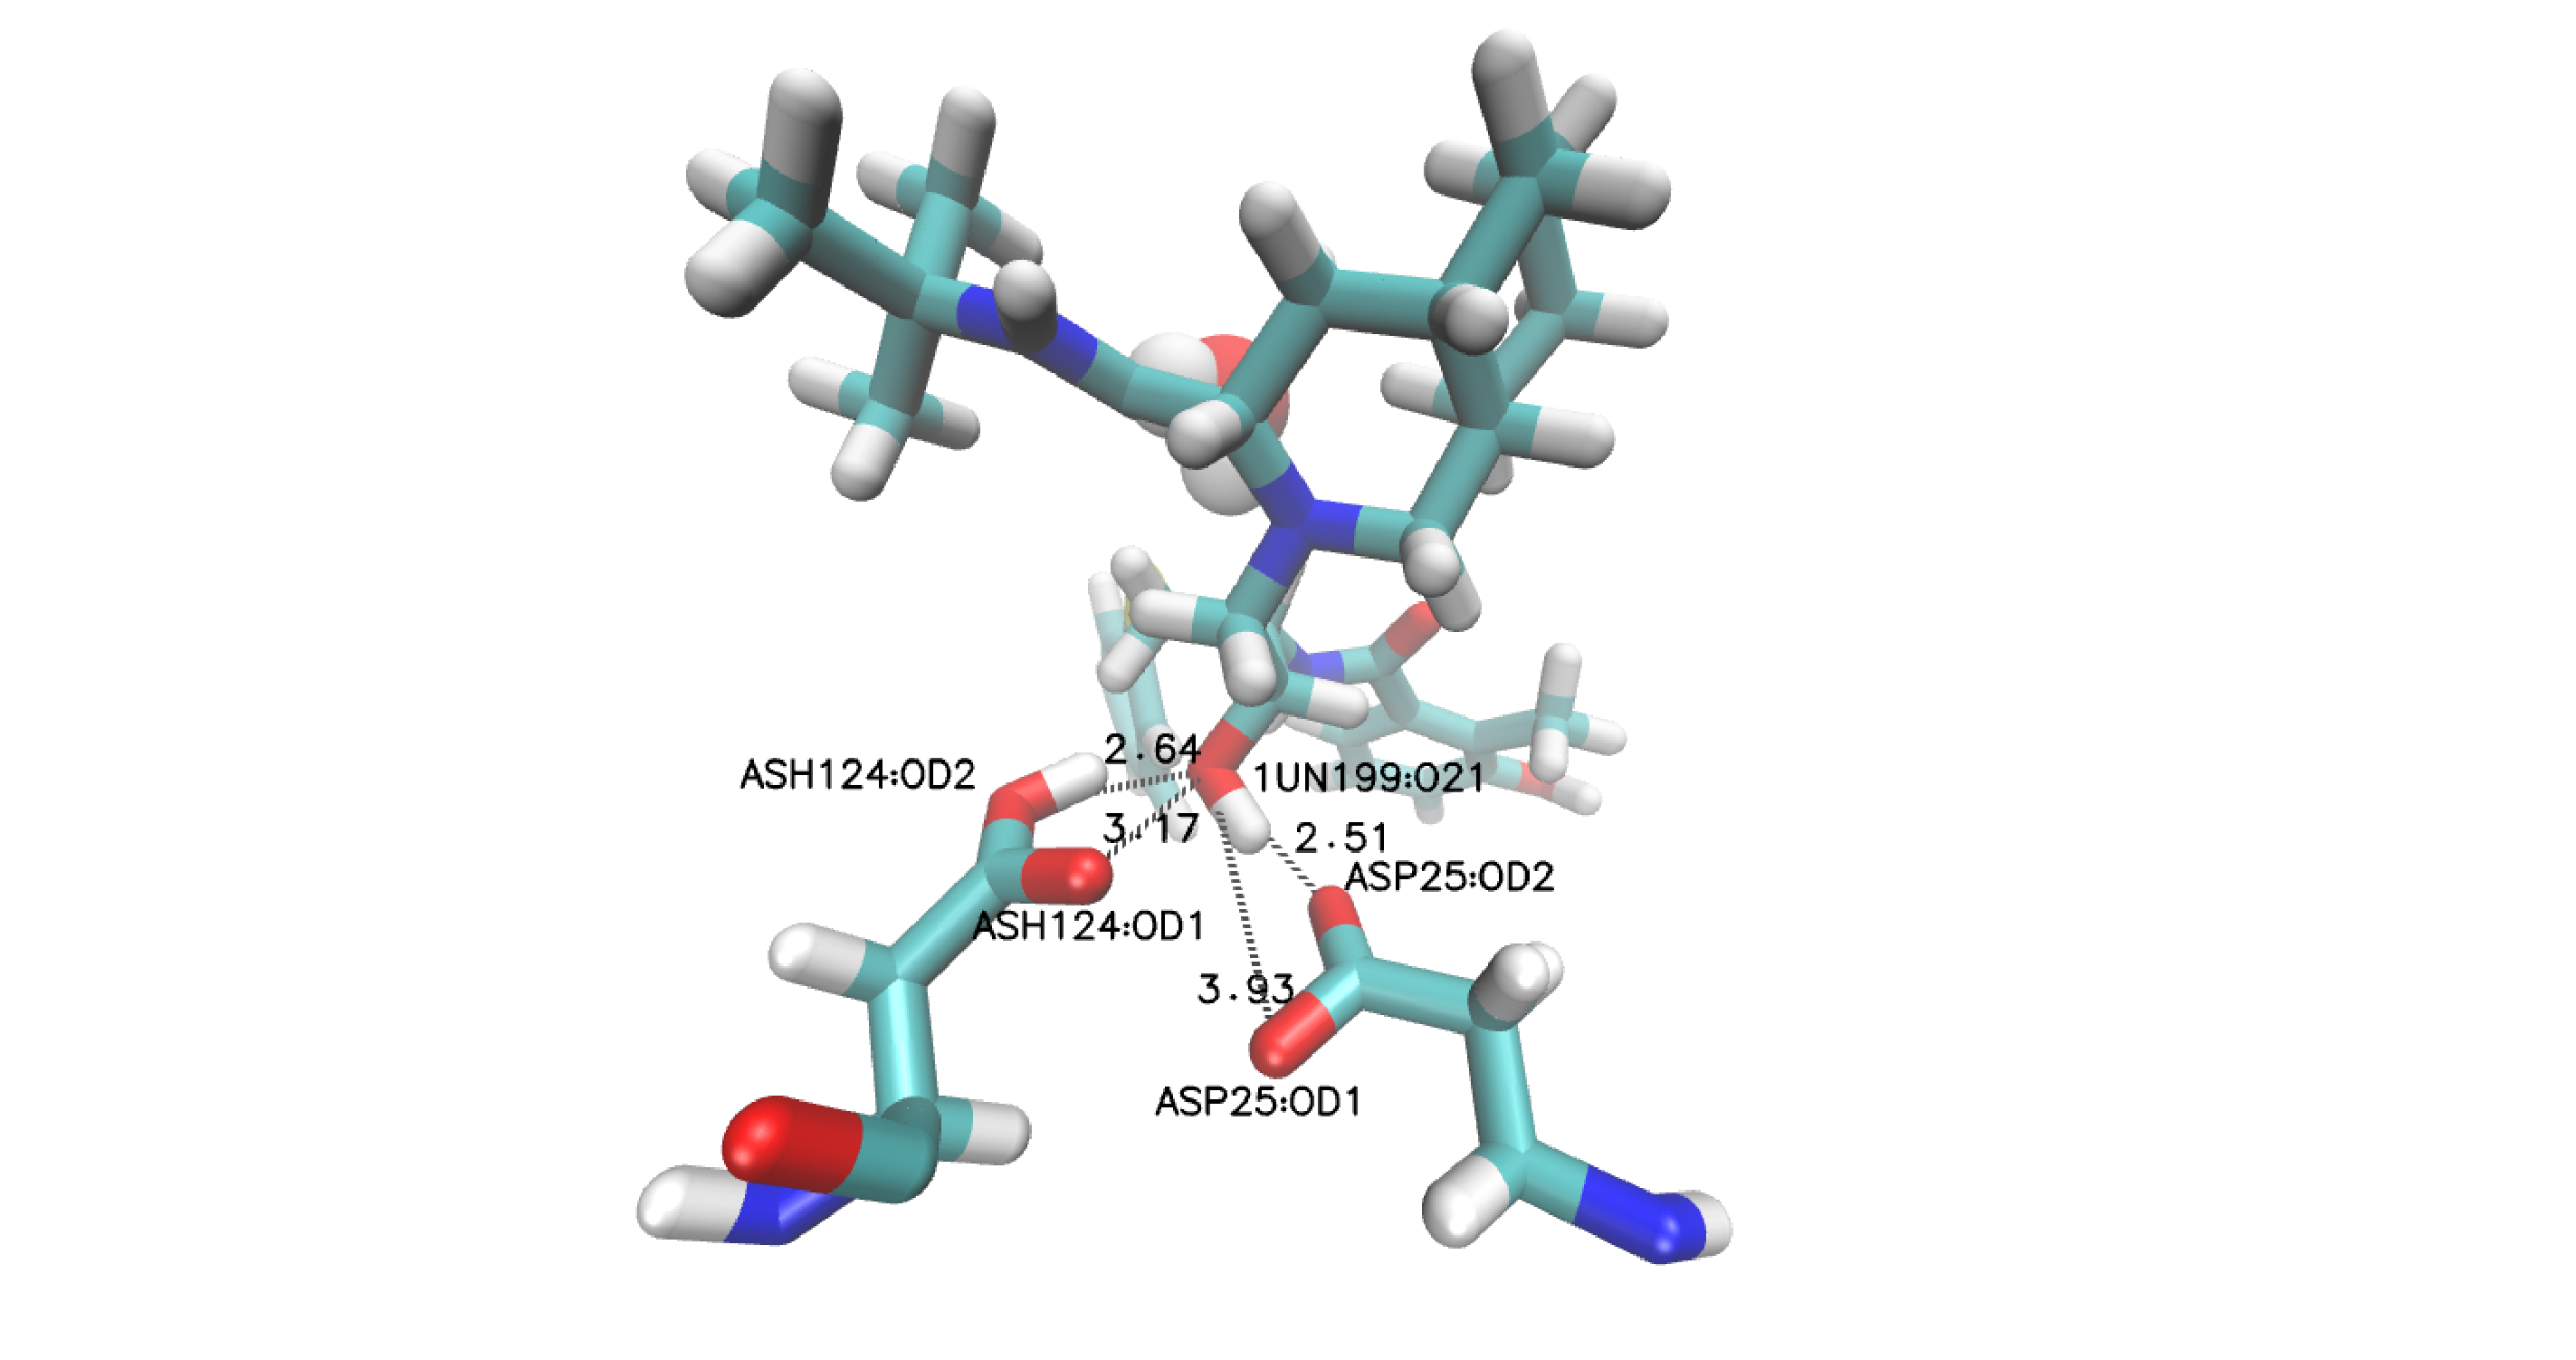
\includegraphics[width=\textwidth]{images/ASPs-distances.png}
			\caption{}
			\label{fig:an:dists-vmd}
		\end{subfigure}
		\begin{subfigure}[b]{0.64\textwidth}
			\centering
			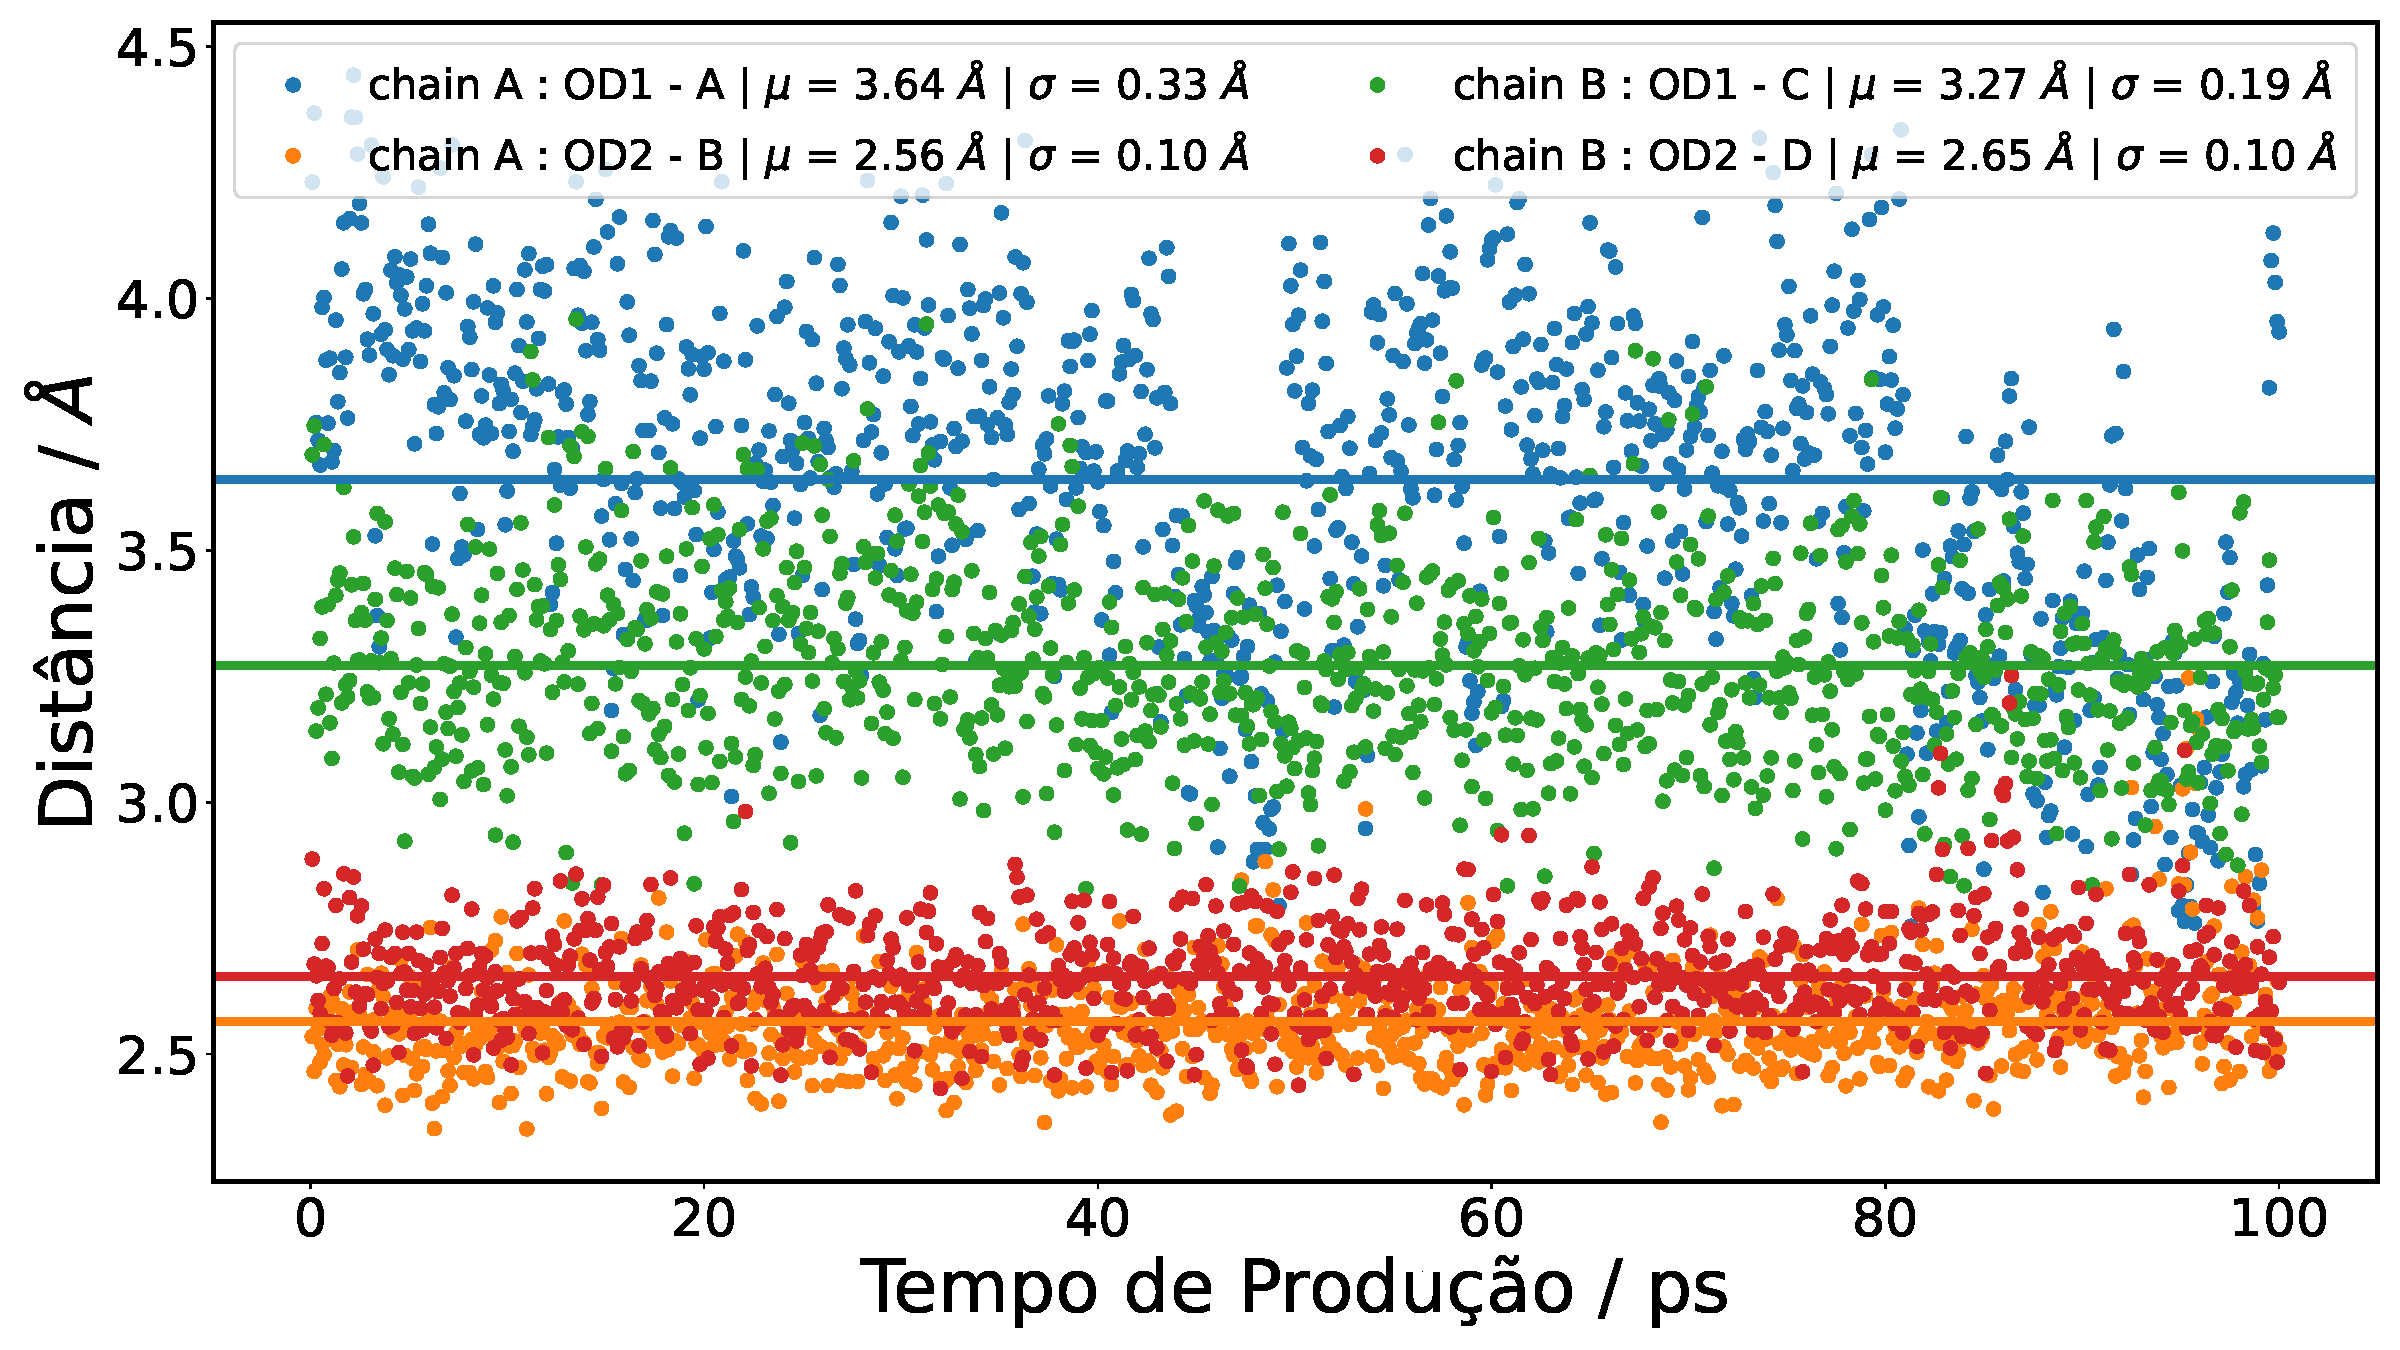
\includegraphics[width=\textwidth]{images/plots-ASP-1UN.pdf}
			\caption{}
			\label{fig:an:dists-plot}
		\end{subfigure}
		\caption{\textbf{(a)} Representação das ligações entre os átomos OD* dos ASP25 ao O21 do inibidor. \textbf{(b)} Gráfico das distâncias (\AA) em função do tempo de produção (ps). Na legenda pode-se observar o valor médio ($\mu$) e o desvio padrão ($\sigma$) dos comprimentos de ligação. Na vertical também estão assinaladas, nas suas cores correspondentes, linhas que correspondem ao $\mu$ de cada ligação.}
		\label{fig:an:ASP-1UN}
	\end{figure}

\section{Conclusões}
	Neste trabalho foram exploradas os primeiros passos com rumo à simulação de sistemas biológicos, tendo sido abordada teoria, trabalho computacional e vários métodos de análise da dados.
	
	A incorporação do Nelfinavir na HIV-1 protease foi o nosso objeto de estudo e foi realizada uma pequena simulação de 120 ps de Dinâmica Molecular, que se mostrou termodinamicamente estável, embora uma estrutura convergida só fosse possível atingir para simulações superiores a 3 ns.
	
	A estrutura final e a sua evolução ao longo da etapa de produção foi analisada à luz das suas propriedades termodinâmicas, \textit{root mean square deviation} e função de distribuição radial (RDF).	Foram também analisadas todas as pontes de hidrogénio do sistema, num total de 202 detetadas, com ênfase atribuída às que uma molécula de água estrutural estabelece com o Nelfinavir e a proteína. Finalmente, foram analisados os comprimentos de ligação entre os ácidos aspárticos do centro ativo da proteína e o inibidor.
	
	Em geral, achei todo este trabalho extremamente interessante e enriquecedor. Tive a oportunidade de aprender fundamentos de uma área que achava ser completamente ortogonal à Física mas que se veio a revelar ter imensa coisa em comum. Gostei do desafio de investigar conceitos como a protonação dos ASP25 no início do trabalho. No entanto, gostava de ter explorado mais a fundo outros pontos como as RDFs e a análise das pontes de hidrogénio, mas sinto que ter frequentado esta cadeira e escrever este relatório me proporcionaram a curiosidade e confiança para investigar estes assuntos por conta própria.
	
	Muito obrigado aos professores pelas ótimas aulas, por promoverem a discussão com os alunos e estarem sempre disponíveis para esclarecer dúvidas.
\newpage
\bibliographystyle{unsrt}
\bibliography{biblio,biblio-vmd}
\end{document}


























\begin{equation}
	U_{\text {intra }}\left(r,\theta,\phi\right)=\sum_{\text {bonds }} K_{\textrm{lig}}\left(r-r_{e q}\right)^{2}+\sum_{\text {angles }} K_{\theta}\left(\theta-\theta_{e q}\right)^{2}+\sum_{\text {dihedrals}} \sum_{n} \frac{V_{n}}{2}[1+\cos (n \phi-\gamma)]+\ldots
\end{equation}